\documentclass[twoside,single]{lion-msc}

\title{Electrochemically changing potential}
\author{Sebastiaan Van Mulken}
\studentid{0950815}
\supervisor{Biswajit Pradhan \\ \hspace*{\fill}Michel Orrit}
\corrector{To be determined}

\begin{document}
\maketitle



\chapter{Introduction}
With the help of single-molecule fluorescence detection methods, optical studies have made many breakthroughs in the field of science. Single-molecule fluorescence resonance energy transfer (FRET) is one of the most general accepted techniques. Different kind of kinetics of proteins, such as redox switching \cite{Akklc}, have been revealed. This switching can be achieved either chemically or electrochemically. Previously, this switching was monitored chemically by adjusting the concentration of oxidizing or reducing agent. In this thesis a new setup is built and tested to achieve switching of proteins electrochemically. Instead of adjusting the concentration of oxidizing or reducing agent a potentiostat will change the potential. This allows more precise and faster changing potentials. With the help of this setup the midpoint potential of blue copper azurin (CuAz) labeled with ATTO655 (position K122) has been determined. 

This thesis does not only show the results of the new setup, but also shows some insights of how the setup was established. Not only does it describe the parts that did work, but also the parts that were not successful. 


\chapter{Theory}
In this chapter, the fundamental physics and electrochemistry are explained which are used in the set up.

\section{Fluorescence}
Fluorescence is the property of certain atoms and molecules to absorb light at particular wavelengths and emit light at longer wavelengths. These type of atoms and molecules are called fluorophores or fluorescent dyes. A brief interval after absorption - the fluorescence lifetime - the atoms or molecules will emit light of less energy (longer wavelengths).  Fluorescence is a process governed by three events. All these events occur on different timescales separated by several orders of magnitude. These events are summarized in Figure \ref{fluor}.
\begin{figure}[ht!]
\centering
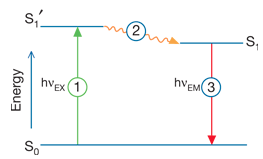
\includegraphics[width=90mm]{fluorescence.jpg}
\caption{The three major events in fluorescence: excitation (1), relaxation (2) and emission (3).} 
\label{fluor}
\end{figure}

\subsection{Excitation}
The first event is excitation. For any molecule, several electronic states exist depending on the total electron energy and the symmetry of the electron spin states. Each state is divided in sub-states - a number of vibrational and rotational energy levels associated with the atomic nuclei and the bonding orbitals. At room temperature, most molecules lack the internal energy to exist in any other state than the lowest vibrational level of the ground state. This ground state is usually an electronic singlet in which all electrons are spin-paired (opposite spins). With the help of a laser, photons with energy $E_{photon}=h \nu_{laser}$ are absorbed by the fluorophores. The absorption of energy happens to any of the closely spaced vibrational and rotational energy levels of the excited states. Absorption of light occurs in a few femtoseconds ($10^{-15}s$). It will only occur for specific wavelengths known as the absorption bands. If a photon contains more energy than necessary for an electronic transition, the excess energy is converted into vibrational and rotational energy via non-radiative processes. If the energy of a photon is too low, no transition occurs. Excitation of a molecule by absorption normally happens without a change in electron spin-pairing. Therefore, the excited state is also a singlet. Usually the fluorophores are excited to higher vibrational levels of the first or second singlet electronic energy state. Certain transitions have higher probability than others and combined they form an absorption spectrum of the molecule.

\subsection{Vibrational relaxation}
After absorption, several processes occur with varying probabilities. The most likely is relaxation to the lowest vibrational energy level of the first excited state, a process known as internal conversion or vibrational relaxation. This is a loss of energy in a non-radiative matter and has a timescale of a picosecond ($10^{-12}s$) or less. Since a significant number of vibration cycles happen during the excited lifetimes, molecules undergo complete vibrational relaxation. The excess vibrational energy is converted into heat, which is transferred to the neighboring solvent molecules.

\subsection{Emission}
The excited molecule exists in the lowest excited singlet state for a period in the order of nanoseconds ($10^{-9}s$) before relaxing to the ground state. During this relaxing, a photon will be emitted. Because the ground state consist of closely spaced vibrational energy levels, the resulting emission intensity is distributed over a band of wavelengths rather than a sharp line. Most fluorophores can repeat the excitation and emission cycle a lot of times. However, the excited state is more reactive with the surrounding which can result in photobleaching: the molecule is permanently unable to fluoresce. 

Other relaxation pathways compete with the fluorescene emission process. The excited state energy can be dissipated as heat, the excited molecule can collide with another molecule to transfer energy (for example quenching) or intersystem crossing to the lowest excited triplet state can occur. The latter will result in emission of a photon through phosphorescence or a transition back to the excited singlet state that yields delayed fluorescence. Molecules who exhibit the triplet state have a high degree of chemical reactivity, often resulting in photobleaching. 

\section{Fluorescence Resonance Energy Transfer}
Fluorescence resonance energy transfer (FRET) permits determination of two molecules within several nanometers, the distance close to where molecular interactions occur. The process of resonance energy transfer can take place when the donor fluorophore in an electronically excited state transfer its excitation energy to a nearby chromophore (the acceptor). If the fluorescence emission spectrum of the donor molecule overlaps the absorption spectrum of the acceptor molecule and the two are within minimal spatial radius, the donor can transfer its excitation energy in a non-radiative fashion through dipole-dipole intermolecular coupling. Treating an excited fluorophore as an oscillating dipole, it can undergo energy exchange with a second dipole having a similar resonance frequency. If the acceptor itself is a fluorochrome, increased or sensitised fluorescence emission is observed. By exciting the donor and acceptor molecules with light of wavelengths centred near the absorption maximum of the donor, the detected light will be emitted at wavelengths centred near the emission maximum of the acceptor if FRET has taken place. This resonance energy transfer is not sensitive to the surroundings of a fluorophore. The FRET efficiency is given by:
\begin{equation}
E = \frac{1}{1 + (r/R_{0})^{6}}
\end{equation}
where $r$ is the distance between the donor and acceptor molecule and $R_{0}$ is the F\"oster distance - the distance at which the energy transfer efficiency is 50\%. Related to this efficiency is the lifetime ($\tau_{D}^{'}$ in pressence of an acceptor and $\tau_{D}^{'}$ with the absence of an acceptor) and the fluorescence intensity ($F_{D}^{'}$ in pressence of an acceptor and $F_{D}$ with the absence of an acceptor) via the formulas
\begin{equation}
E = 1 - \frac{\tau_{D}^{'}}{\tau_{D}}
\end{equation}
and
\begin{equation}
E = 1 - \frac{F_{D}^{'}}{F_{D}}.
\end{equation}


\section{FluRedox principles and labelled azurin}
In contrast to FRET, FluRedox is based on the change of the overlap integral associated with a change in the optical properties of the redox-active centre upon oxidation and reduction. The optical read-out responds exclusively to the redox state of the protein \cite{Akklc}. 

Azurin is a blue copper protein with an active copper site (see Figure \ref{azurin}). The active centre of azurin has strong characteristic features in its optical absorption spectrum which is dependent on the redox state. It may occur in oxidised ($\textup{Cu}^{2+}$) or reduced ($\textup{Cu}^{+}$) form. Oxidised azurin exhibits a strong absorption band around 600 nm (blue). Fluorescent labelling of this protein makes it suitable for single molecule studies. ATTO-655 is a fluorescence dye with a emission band around 680 nm. The emission band of the dye and the absorption band of the azurin overlap (see Figure \ref{absorption}). When azurin is oxidised, FRET between the dye and the centre quenches the dye fluorescence. This quenching is absent when the protein is in reduced state because its 600 nm absorption has vanished \cite{Tabares2014}.

\begin{figure}[ht!]
\centering
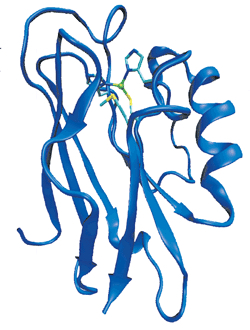
\includegraphics[width=50mm]{azurin1}
\caption{Three dimensional structure of azurin. The green sphere is the copper centre of the protein. Picture is taken from \cite{BORMAN2010}.} 
\label{azurin}
\end{figure}

\begin{figure}[ht!]
\centering
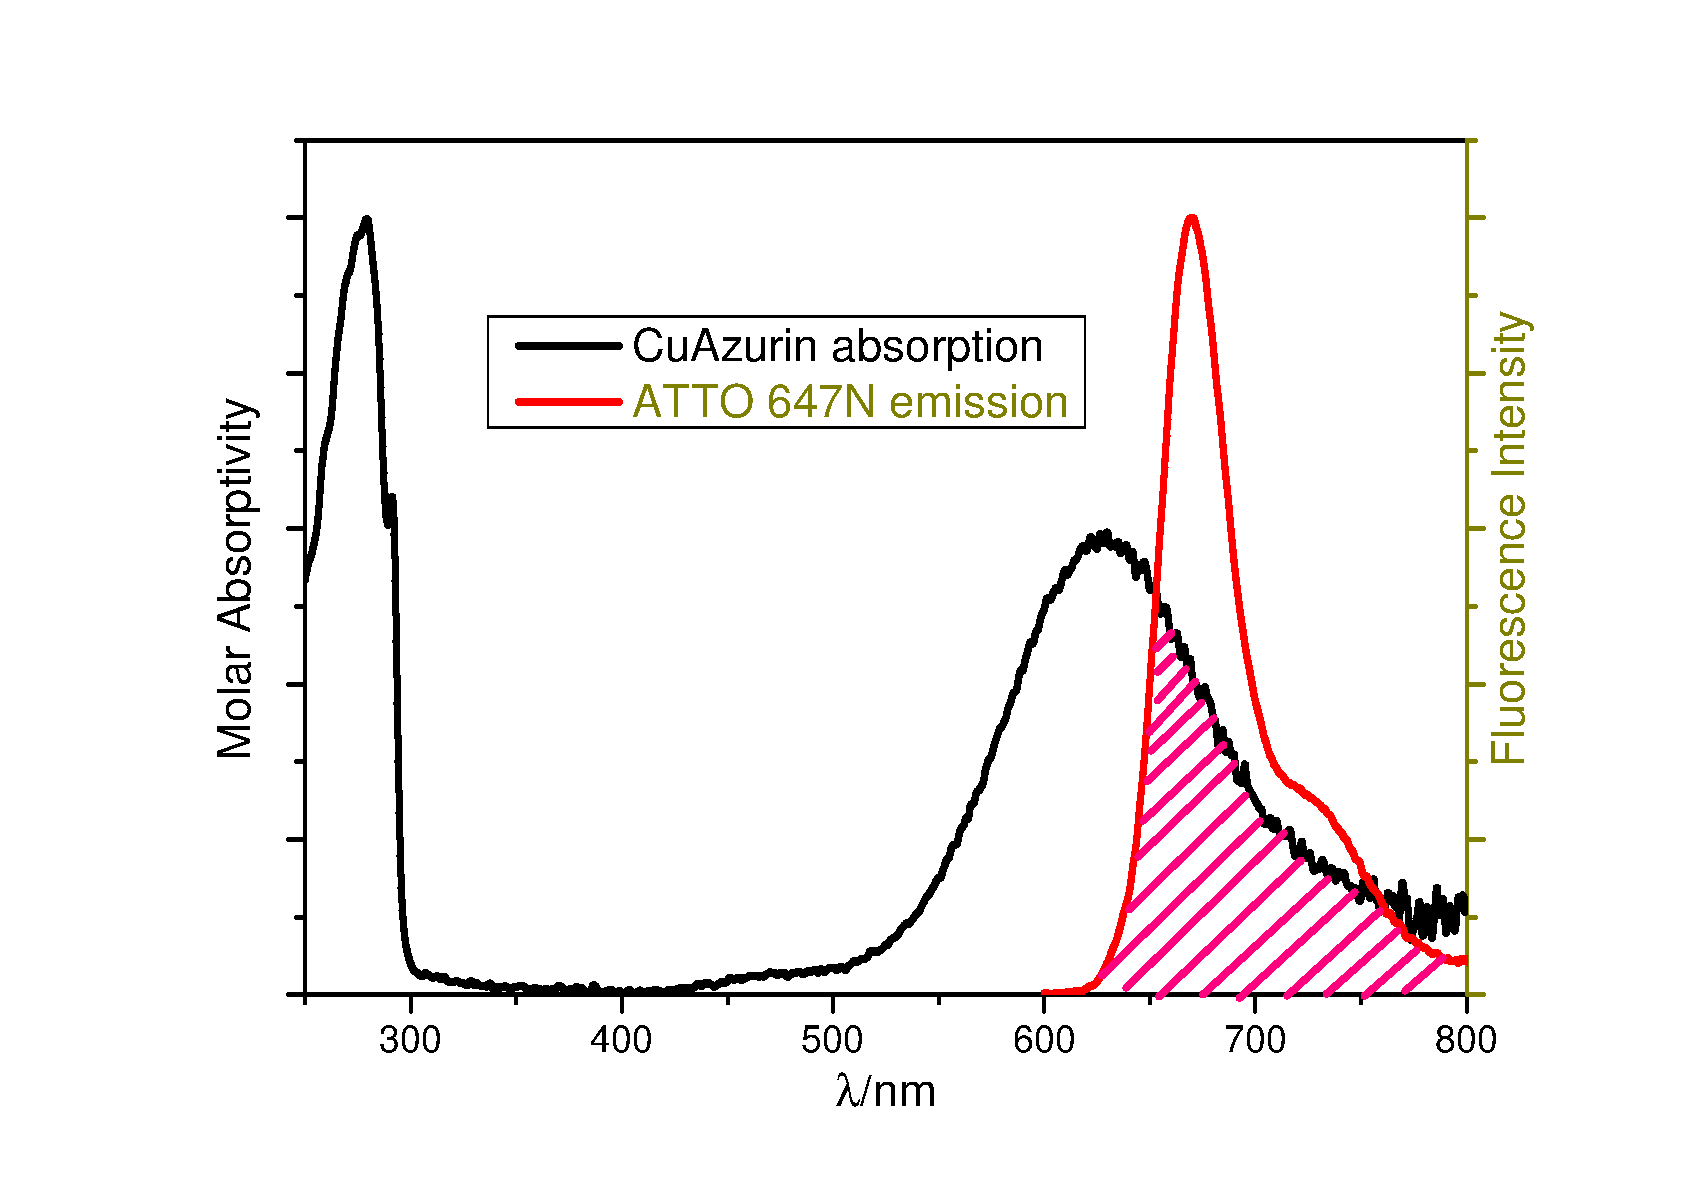
\includegraphics[width=90mm]{absorp.pdf}
\caption{Absorption spectrum of CuAz (black) and the emission spectrum of the fluorescence dye ATTO-655 (red). The overlapping parts are purple marked. The absortion band around 600 nm is absent when azurin is reduced.} 
\label{absorption}
\end{figure}


\section{Single molecules techniques}
It is impossible to open newspapers without stumbling over words that reflect the impact of life sciences to the modern world. Many speculations and discussions suffer from vagueness since many biological mechanisms are barely known to exist and even less mechanisms are fully understood. New and more precise techniques have made this field grow quickly. With new synthetic fluorophores, the ability to study single proteins at a time is exploited to investigate a variety of dynamics.  One of the ways to get a better understanding of these single proteins is the usage of fluorescence correlation spectroscopy and the usage of confocal microscopes. 

\subsection{Fluorescence Correlation Spectroscopy}
The instrumentation of Fluorescence Correlation Spectroscopy (FCS) is based on an inverted confocal microscope.  A laser beam is directed into a microscope objective via dichroic mirrors and focused on the sample. High numerical aperture are used. Fluorescence light from the sample is collected and passed through the dichroic and emission filter. A pinhole in the image plane blocks the light not originating from the focal region. When concentrations in order of a few - or less - nanomolar of fluorescent particles are applied, single particles can be monitored at a given time. A more detailed description can be found in reference \cite{Schwille}.

The fluorescence intensity collected during the experiments were elaborated using the normalized autocorrelation (AC) function, defined by:
\begin{equation}
G'(\tau) = \frac{\left \langle I(t)I(t + \tau) \right \rangle}{\left \langle I(t)\right \rangle ^{2}}.
\end{equation}
Substracting the normal offset of value 1, this leads to
\begin{equation} \label{AC}
G(\tau) = G'(\tau) - 1 =  \frac{\left \langle \delta I(t)\delta I(t + \tau) \right \rangle}{\left \langle I(t)\right \rangle ^{2}}
\end{equation}
where the brackets  denotes temporal averaging and $\delta I(t) = I(t) - \left \langle I(t)\right \rangle$. The autocorrelation function is used to compute the self-similarity after lag-time $\tau$.

\subsection{Confocal Laser Scanning Microscopy}
Confocal Laser Scanning Microscopy (CLSM) is the setup we used in this experiment. The CLSM is used to scan a sample. In contrast to the FCS, the detection of the signal from the sample depends on strategic choices. The sample is mounted on a moving piezoelectric scanning stage. This allows sub-micrometer movements. The scanning stage is moved along the confocal volume and the fluorescent signal is collected for each position sampled. Together with the fluorescence intensity, the setup is equipped to record the lifetime of the fluorescence and timetraces with the help of a time-correlated single-photon counting (TCSPC) board. A more detailed description of the setup is found in sections \ref{confo_micro} and \ref{data_coll}.

For this thesis, the Cu-azurin and Zn-azurin were labeled and immobilized on the sample slide. Surrounded by an electron mediator, different potentials were applied on areas of (20 x 20) $\upmu \textup{m}^{2}$, which have around 30 - 40 immobilized proteins. Initially applying a positive and negative potential, by means of lifetime analysis and intensity, the active azurin and inactive azurin/impurities can be pointed out directly after taking the images, since the FRET effect affects directly the lifetime of the dye (see Figure \ref{finding_proteins}). Once we select the working proteins, the signal of the proteins is recorded for different time intervals (usually 30 seconds) resulting in timetraces as showed in Figure \ref{TT_exam}.

\begin{figure}
\begin{subfigure}{.5\textwidth}
  \centering
  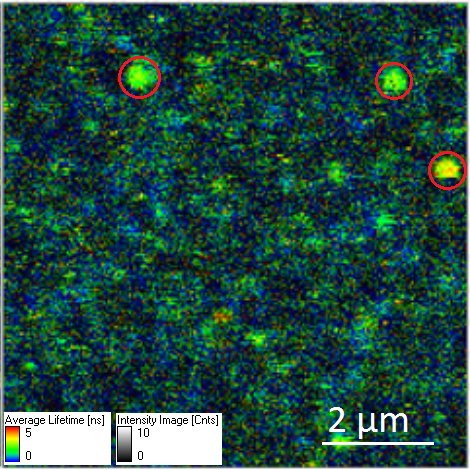
\includegraphics[width=.95 \linewidth]{voorbeeld_protein_2}
  \label{}
\end{subfigure}%
\begin{subfigure}{.5\textwidth}
  \centering
  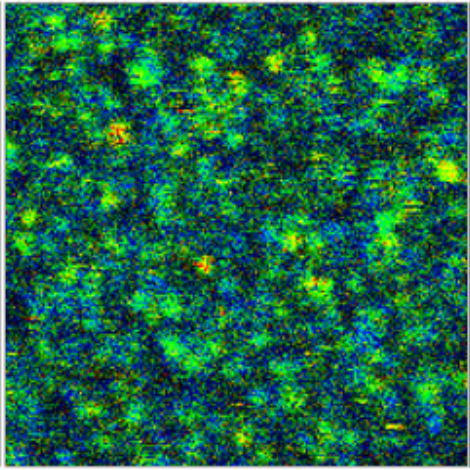
\includegraphics[width=.95 \linewidth]{voorbeeld_protein_1}
  \label{}
\end{subfigure}
\caption{A  (10 x 10) $\upmu \textup{m}^{2}$  area filled with immobilized Cu-azurin at different potentials. On the left: potential of 100 mV, here the Cu-azurin is oxidized. The bright spots (red circles) are either bleached proteins or impurities. A way to get rid of these impurities is by focussing the laser with slightly more power on these spots. On the right: same area, but with -100 mV potential. All the proteins are reduced. Comparing these two pictures show immediately the active protein and the non active proteins/impurities.}
\label{finding_proteins}
\end{figure}


\begin{figure}[ht!]
\centering
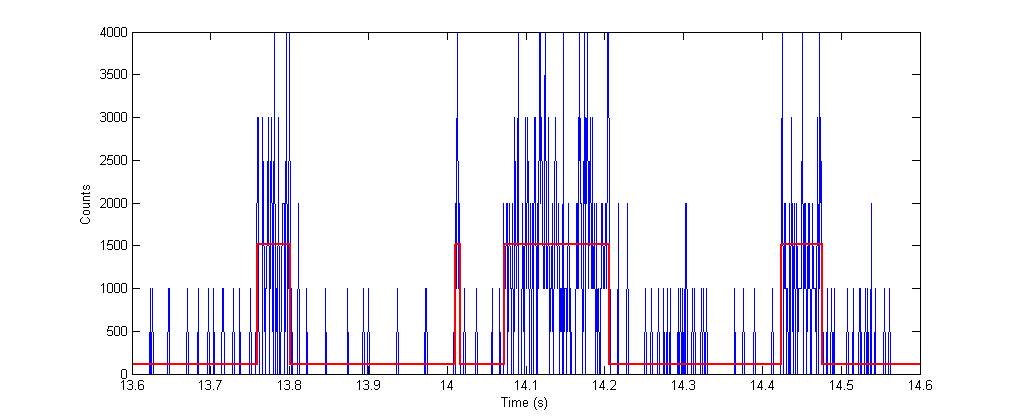
\includegraphics[width= \textwidth]{TT_example}
\caption{Example of a small part of a 30 sec timetrace of an immobilised Cu-Azurin in a -100 mV potential, taken with a CLSM. The blue line is the raw data, the red line is the fitted on and off magnitude and changepoint times. This is calculated using a specific program which is in more details described in the Data section.} 
\label{TT_exam}
\end{figure}

\section{Binding protein to the surface}\label{neutra}
In a variety of different applications the biotin-avidin system has been used \cite{Diamandis1991}. Living organisms develop highly specific defence mechanisms to help survive in unfriendly environments. Avidin, a protein found in egg white, has the ability to bind with very high affinity to vitamin biotin. This interaction is thought to represent the natural defence mechanism: the binding of avidin with biotinylated enzymes inactivates the enzymes.and thus inhibits the growth of bacteria. Compared to other  ligand-binder interactions, biotin-avadin has unique characteristics. The nonconvalent interaction of avadin with biotin has a formation constant of $10^{15}\textup{L}\cdot \textup{mol}^{-1}$, much greater than the interaction of ligands with their specific antibodies (about $10^{3}-10^{6}$ times greater). Also the avidin to biotin binding is specific enough to ensure the binding direct to the target of interest. Finally, the avidin possesses four binding sites per molecule. 

The NeutrAvidin is used unlabelled and serves as a link between the biotinylated binder (the biotin on the glass slide) and the biotinylated molecule (labeled Cu-azurin). This is illustrated in Figure \ref{avadinbinding} 

\begin{figure}[ht!]
\centering
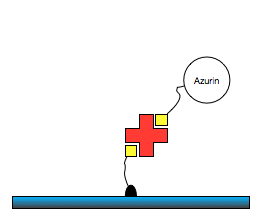
\includegraphics[width=70mm]{avadin}
\caption{Illustration of the sample slide - NeutrAviding - protein binding. The red cross is the NeutrAvidin, with the four corners representing the binding spots for biotin. The yellow rectangulars represent the biotin. One side is bound to the glass surface while the other side is connected to the azurin}
\label{avadinbinding}
\end{figure}


\section{Oxidation-reduction reactions}
Electron transfer (ET) is the movement of electrons and can be generated by movements of electrons from one element to another in a oxidation-reduction (redox) reaction. Oxidation is the loss of electrons, reduction is the acquisition of electrons. The species being oxidized is called the reductant and the species being reduced is called the oxidant. The oxidation-reduction reaction can occur spontaneously. This is due to the difference in potential energy between the two substances. This difference is called the cell potential, denoted as $E_{cell}$. This cell potential depends upon the concentration of species as well as temperature. The greater the cell potential the greater is the driving force of the electrons. Since the standard state cell potential $E^{0}_{cell}$ is measured under standard states (1 Molar and 1 atmospheric pressure), it differs from the non-standard state cell potential. The two are closely related via
\begin{equation} \label{nernst}
E_{cell} = E^{0}_{cell} - \frac{RT}{nF} \ln Q
\end{equation}
or in terms of $\log_{10}$
\begin{equation}
E_{cell} = E^{0}_{cell} - \frac{0.0592}{n} \log_{10} Q
\end{equation}
where Q is the reaction quotient. This equation is referred to as the Nernst equation. For a reversible reaction (which is usually the case in redox reactions) $\textup{aA + bB}\rightleftharpoons\textup{cC + dD}$ where a, b, c and d are the stoichiometric coefficients for the balanced reaction, we can calculate the reaction quotient using:
\begin{equation}
Q=\frac{\left [\textup{C}  \right ]^{a}\left [\textup{D}  \right ]^{d}}{\left [\textup{A}  \right ]^{a}\left [\textup{B}  \right ]^{b}}
\end{equation}

\section{Electrochemical detection}
Electrochemical detection instruments can be used for monitoring the current passing through a flow cell in liquid electrochemistry and flow injection analysis, but they can also be used for other electroanalytical applications. The potential control range of these instruments is $\pm10V$. To reach certain potentials, a constant potential is applied and the current is recorded as function of time (amperometric i-t curve), as is shown in Figure \ref{amp_curve}. Once the current in the i-t Curve is constant (i.e flat), the solution has reached the demanded potential. The data sample interval is chosen according to the length of the experiment.


\begin{figure}[ht!]
\begin{subfigure}{.5\textwidth}
  \centering
  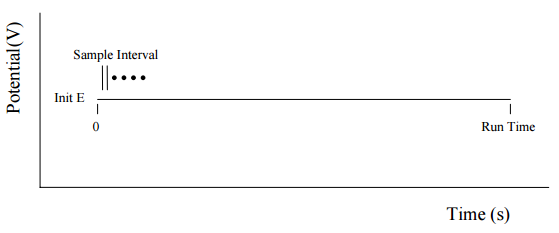
\includegraphics[width= \textwidth]{amp_curve}

  \label{}
\end{subfigure}%
\begin{subfigure}{.5\textwidth}
  \centering
  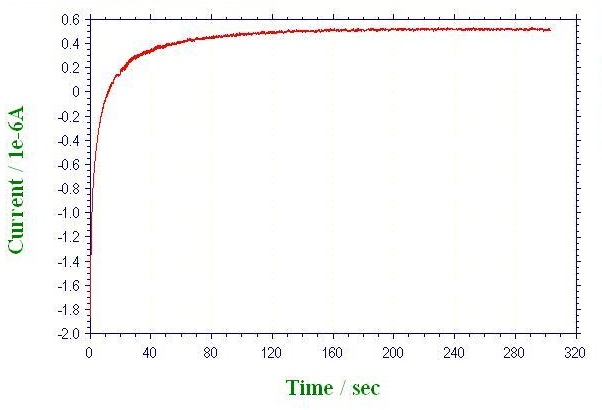
\includegraphics[width=.95 \linewidth]{it100mV}
  \label{}
\end{subfigure}
\caption{The amperometric i-t curve.  Right: the i-t curve of oxidizing conditions. The curve goes flat within minutes allowing change in potential in relative short time scales.}
\label{amp_curve}
\end{figure}



\chapter{Experimental setup}

This chapter covers the establishment of the setup from the start till the end. In papers and publications, it is not  common to describe how the experiment was built from the start till the end, but considered the duration and effort it took during this project it cannot be excluded from this thesis. The chapter is divided in three parts: the first part describes the previously used setup in which the potential changed chemically by increasing or decreasing the concentration of  electron donor. The second part of this chapter covers the progress from scratch to the final setup including the experimental successes and experimental failures. The final part of this chapter discusses the final setup and how it operates. It is this setup with which the data is acquired.

Some parts and techniques such as the confocal microscope and functionalizing of the glass slides is used in both setups. Therefore these are described below.

In this chapter and the rest of the thesis: the blue copper azurin used in the experiments is  labeled with ATTO665 at binding site K122 (lysine at position 122). When copper azurin (CuAz) is mentioned, it is referred to the one with ATTO665 label.
The potentials measured and mentioned in this thesis are always with respect to the calomel electrode.


\section*{Confocal microscope}  \label{confo_micro}
To perform the experiment, a home built confocal microscope used previously for similar experiments \cite{Gupta2014} was used. A 639 nm pulsed laser, controlled by a PDL 800-B (PicoQuant) laser driver at 40MHz repetition rate, is passed through a narrow band filter (LD01-640/8-25, Semrock). To collimate the beam to the desired diameter an aspheric lens of suitable focal length was used. The beam then got reflected via a dichroic mirror (ZT640RDC, Chroma) to the high numerical aperture (NA) oil immersion objective (1.4 NA, 100X oil, Zeiss). The stage on which the sample was mounted was controlled by a nanopositioning piezo element (P517.3CD, Physic Instrumente). The emission was collected and filtered through an emission filter (ET655LP, Chroma) and focused onto a $50\upmu \textup{m}$ pinhole to filter the background. Once the beam got focused on the active area of a single photon counting module (SPCM-AQR-14, Perkin Elmer) data acquisition was performed by a photon counting PC-board (TimeHarp 200 PicoQuant). A schematic set up is shown in Figure \ref{micros}.

\begin{figure}[ht!]
\centering
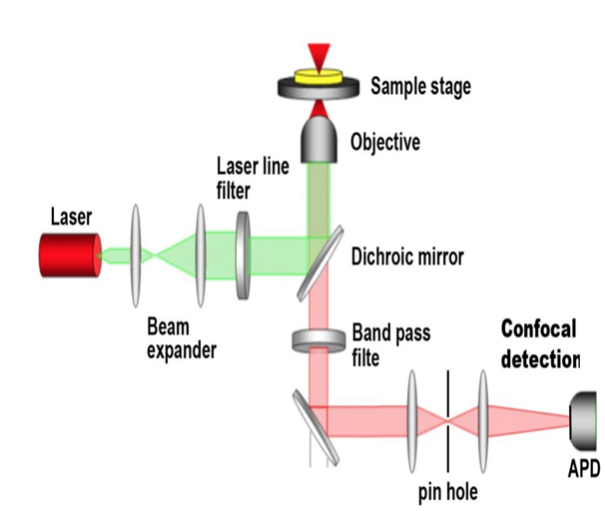
\includegraphics[width=70mm]{schem_micros}
\caption{Schematic drawing of the confocal microscope used in the chemical and electrochemical set up. }
\label{micros}
\end{figure}


\section*{Functionalizing glass slides}
Not only the same confocal microscope was used in both setups, also the immobilization of the proteins is similar. The functionalization of the cover glass is based on the process used in \cite{Gupta2014}.  \diameter 25mm \#1 thickness glass coverslips (Menzel-Glaser) were used for all immobilizations. The coverslips were rinsed several times with milliQ water and treated with a  $\textup{H}_{2}\textup{O} / \textup{NH}_{4}\textup{OH} / \textup{H}_{2}\textup{O}_{2}$ (5:1:1) bath at 70$^{\circ}$ C. The coverslips were then rinsed again but with water and finally with ethanol. The result of this process is the coverslips contain active silanol groups which can react with silanes and thus providing capability to functionalize the surface. The coverslips were stored in ethanol.


Before usage, the coverslips were flamed and then ozone cleaned for 15 minutes. Then the coverslips were treated for 30 min with a 1\% solution of 3-(2-aminoethyl)aminopropyl trimethoxysilane in methanol containing 5\% glacial acetic acid. After washed extensively with methanol, the coverslips were sonicated with intervals of 10 minutes. Dried with clean nitrogen, it was left in the desiccator overnight or kept in the oven at 65$^{\circ}$ C for 3 hours. The next day they were treated with a 5 mg/mL solution of methoxy-peg-NHS (MW 2000, Laysan Bio) and 0.05 mg/mL biotin-peg-N-hydroxysuccinimide (MW 3400, Laysan Bio) in 50mM phosphate buffered saline (PBS)  with pH 7.4. To ensure enough biotin functionalities are present the ratio of biotin peg to methoxy was kept at 1:100 in the final experiments.  






\section{Changing the potential chemically}\label{pot_chem}

A small glass slide is functionalized in a similar way explained previously. A syringe is used to suck solution through the tubes onto the glass slide. One side is connected to the syringe, the other side is connected to the desired solution. First a mixture of proteins is put on the glass slide. After sufficient time, the proteins will bind to the glass slide. A new mixture consistent of buffer HEPES (pH = 7) is then sucked through the tube onto the glass slide to remove non-bound proteins. Once the proteins are removed, a new mixture consistent of ascorbate ($\textup{C}_{6}\textup{H}_{8}\textup{O}_{6}$) and potassium ferricyanide ($[\textup{Fe(CN)}_{6}]^{4-}$) is incubated into the flow cell. Ascorbate is an antioxidant and exists predominantly as the ascorbate monoanion  $\textup{AschH}^{-}$. The standard potential of ascorbate is around 40 mV (pH = 7) with respect to a colomel electrode, which is close to the standard potential of the proteins. Oxidation of ascorbate forms $\textup{ascorbyl radical Asc}^{\bullet  -}$, the equivalent of ascorbate but with one less proton and one less electron. Upon further oxidation this becomes dehydroascorbate ($\textup{C}_{6}\textup{H}_{6}\textup{O}_{6}$) \cite{Warren2010}. Schematically this becomes:

\begin{figure}[ht!]
\centering
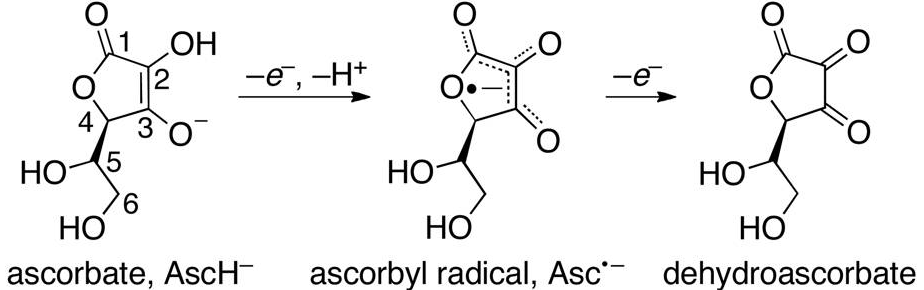
\includegraphics[width=\textwidth]{redox_asc}
\caption{Redox of ascorbate}
\label{redox_asc}
\end{figure}

At equilibrium, using the Nernst equation (Formula \ref{nernst}), the potential can be written as

\begin{equation}
E = E^{0} - \frac{RT}{F} \log_{10} \frac{[\textup{C}_{6}\textup{H}_{6}\textup{O}_{6}][\textup{Fe(CN)}_{6}]^{3-}}{[\textup{C}_{6}\textup{H}_{8}\textup{O}_{6}][\textup{Fe(CN)}_{6}]^{4-}}.
\end{equation}

Thus by adjusting the concentration of ascorbate (in this case adding ascorbate) or ferri-/ferrocyanide, different potentials will be achieved in the solution. The final redox potentials of the solution were measured with a reference electrode (standard calomel, SCE) and a platinum counter electrode connected to a voltmeter.

Some of the downsides to this setup are summed below:
\begin{itemize}
\item The change of potential is induced by adjusting the concentration of ascorbate or ferri/ferrocyanide. By adding or removing substances, the solution will be disturbed. The chance of losing the monitored proteins is substantial if this is not done carefully. 
\item Reaching specific potentials is only possible by adding or removing the exact amount of redox participants. A small mistake and the wanted potential will not be reached. 
\end{itemize}

These downsides lead ultimately to the desire of a better controllable and reliable setup. 

\section{Process to the final setup}

In the previous setup the potential was controlled by adding different concentration of chemicals. In the new setup, these changes are achieved electrically. Beside the confocal microscope, a new instrument has to be introduced: the electrochemical analyzer (Model 800B Series Electrochemical Detector, CH Instruments). Instead of using different concentrations of ascorbate, a cell with a working electrode, counter electrode and reference electrode in a buffer is used. During the process of getting to the final setup, the same working electrode, counter electrode and reference electrode is used: a \diameter250$\upmu \textup{m}$ golden wire acts as the working electrode, the counter electrode is a \diameter0.5mm thin platinum wire and the reference electrode is a saturated calomel electrode. All the potentials throughout this work are reported relative to the SCE.

\subsection{Electron mediator}\label{ferriferro}
When looking at single molecule level, it is expected to see the molecule spend half the time reduced and half of the time oxidized when the potential is set to the mid-point potential of the molecule. This  is evidenced by equal on- and off-times for the blinking. For reducing potentials the molecule will spend more time in the off state and for oxidizing potentials the molecule will spend more time in the on state. It is therefor important to have a range of potentials that are below and above the mid-point potential of the molecule of interest. In the case of Cu-azurin, the midpoint potential is around 25 mV. A solution consistent of a buffer and a redox-pair is needed to act as a electron mediator to obtain the potentials around the mid-point potential of Cu-azurin. A good way to check what range of potentials such solution can reach is the use of cyclic voltammetry (CV) measurement. This is a plot of the current versus the potential. Since the previous setup did not use the potentiostat, the first thing we did for this experiment was using this device to obtain the CV of different solutions to find the one solution that suits this experiment the best.

To obtain the CV of different solutions, a small setup was made. A volume of around 200 mL was put on top of magnetic mixer and the working, reference and counter electrode were lowered into the solution and connected to the potentiostat. With this setup, three different solutions were chosen based on its midpoint potential (see below). It is useful to chose a solution with its midpoint potential close to the midpoint potential of the CuAz, since it is easier to reduce or oxidize near the midpoint potential. For obvious reasons, the interesting potentials in this thesis are the potentials around the midpoint potential of CuAz.
\begin{enumerate}
\item A solution with ascorbate. Arscorbate, together with ferricyanide, is used in the chemically-induced redox switching setup. The details of the redox of ascorbate is described in more detail in section \ref{pot_chem}.
\item With a midpoint potential of 6 mV, the redox couple potassium ferricyanide ($[\textup{Fe(CN)}_{6}]^{4-}$)/ferrocyanide ($[\textup{Fe(CN)}_{6}]^{3-}$) is a close to perfect candidate for this experiment. The oxidation of ferrocyanide, resulting in ferricyanide is given by
\begin{equation}
[\textup{Fe(CN)}_{6}]^{4-}\rightleftharpoons[\textup{Fe(CN)}_{6}]^{3-} + \textup{e}^{-}.
\end{equation}
Following the Nernst equation:
\begin{equation}
E = E^{0}_{\textup{FeCN}} - \frac{RT}{F} \log_{10} \frac{[\textup{Fe(CN)}_{6}]^{3-}}{[\textup{Fe(CN)}_{6}]^{4-}}.
\end{equation}
\item The last solution tested was phenazine ethosulfate (PES). Its midpoint potential is 55 mV and very close to the documented midpoint potential of CuAz. PES in oxidized state may receive electrons from the electrode to get reduced and in closed vicinity the redox potential is controlled by the concentration ratio of $\textup{[PES]}_{ox}/\textup{[PES]}_{red}$. 
\end{enumerate}
In the final setup, the total volume of the solution is 4 mL. When tried to measure the potential of the ferri/ferro redox couple, a volume of 200-300 mL was used. While stirring, oxidizing the redox couple was a fast process. Reducing the ferricyanide, however, took much longer. One explanation could be oxidative stress. Water contains hydrogen in the oxidation state +1 and oxygen in the oxidation state -2. Because of that, the reaction
$$\textup{Fe}^{2+}+\textup{O}_{2}\rightarrow\textup{Fe}^{3+}+\textup{O}_{2}^{-} $$
can occur \cite{Grady1991}. This will slow down the production of $\textup{Fe}^{2+}$ and thus according to the Nernst equation, lower potentials will be reached slower or not at all. Also the setup is not sealed from the air which contains oxygen. In previous voltage-induced redox switching experiments\cite{Akkilic2015} measurements in anaerobic conditions were performed to reduce (in some cases it was reduced to an extend the interaction with oxygen was considered non-existent) the interactions with oxygen. This problem occurred for the other solutions too, but for PES in a lesser extend. Therefore a 200 $\upmu \textup{M}$ PES in PBS with a total volume of 4 mL was chosen as electron mediator in the follow-up experiments.
 

\subsection{Proteins on the surface}
Having functionalized sample slides and a fitting electron mediator, the next phase in the process to the final setup is to get the right amount of proteins on the sample slide. As mentioned in section \ref{neutra},  NeutrAvidin is used as a link between the sample slide and the proteins and has four possible bind spots  (Figure \ref{avidinratio}). Before the proteins were applied on the sample slide, they were mixed together with the NeutrAvidin. Different ratios between proteins and NeutrAvidin were tried to find the right ratio. When more proteins bind to the same NeutrAvidin, the proteins will quench due to collisional quenching. The quencher diffuses to the protein during the lifetime of the excited state. Upon contact, the proteins returns to the ground state, without emission of a photon. The protein and quencher must be in contact \cite{Lakowicz2006}. The quenched proteins visualizes as blue spots on the sample slide (their lifetime is shorter), as is clearly the case when the ratio between proteins and NeutrAvidin was 1:1 (see Figure \ref{finding_proteins}). Lowering the ratio of proteins to the same amount of NeutrAvidin ensures the fact that less protein will bind to the same NeutrAvidin. At some point the probability that the NeutrAvidin is bound to more than one protein is very slim. This is the case when the ratio between protein and NeutrAvidin is 1:40 and this ratio is used in further experiments.

\begin{figure}[ht!]
\centering
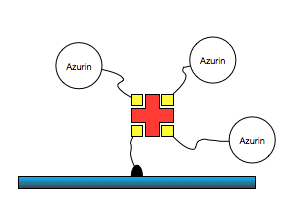
\includegraphics[width=70mm]{ratio_avadin}
\caption{Illustration of NeutrAvidin (red cross) bound to three azurin molecules via biotin (yellow). This is likely the cause of collisional quenching.}
\label{avidinratio}
\end{figure}


\begin{figure}
\begin{subfigure}{.5\textwidth}
  \centering
  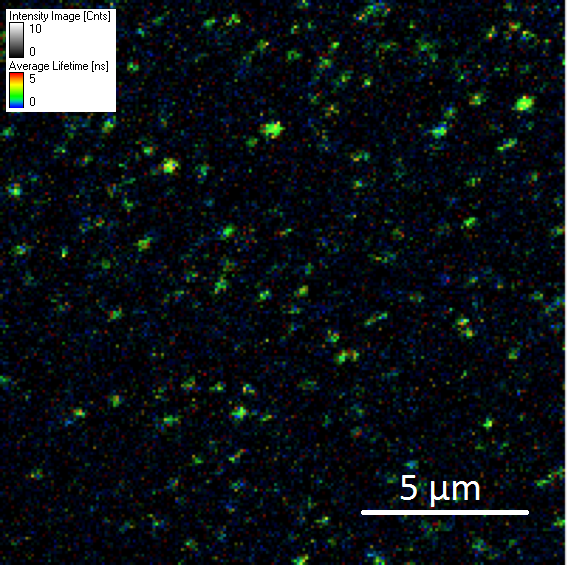
\includegraphics[width=.95 \linewidth]{onetooneratio}
  \label{}
\end{subfigure}%
\begin{subfigure}{.5\textwidth}
  \centering
  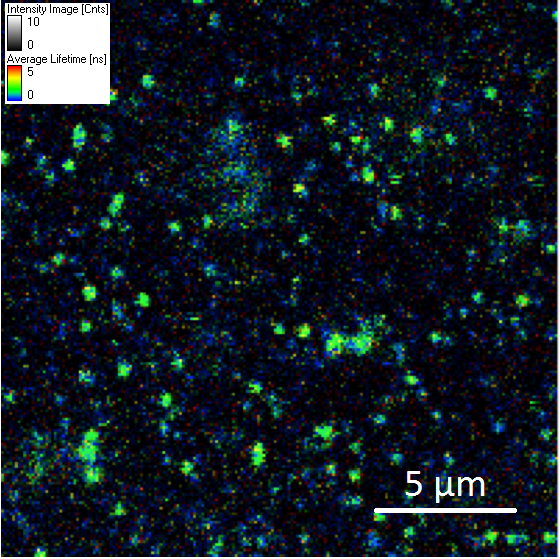
\includegraphics[width=.95 \linewidth]{onetofive}
  \label{}
\end{subfigure}
\caption{A (20 x 20) $\upmu \textup{m}^{2}$ image of immobilised azurin on the sample slide with different ratios of protein to NeutrAvidin. Left: the ratio between protein and NeutrAvidin is 1:1. Right: the ratio between protein and NeutrAvidin is 1:5. When the amount of proteins to NeutrAvidin is decreased, a decreased amount of quenched proteins (blue spots) is observed.}
\label{finding_proteins}
\end{figure}


\subsection{The working electrode}
In an electrochemical system, the working electrode is the electrode of interest. In this case the working electrode is made of gold, since gold is one of the best electron conductors. The reaction of interest is occurring on and near the working electrode in conjunction with the counter electrode and reference electrode. Since the establishment of the redox potential relies on the diffusion of the electron mediator, the actual redox sensed by the molecule is dependent on the distance between the working electrode and the molecule as well as on the time after an external potential is applied. One way to keep the distance between the molecule and working electrode as small as possible is by creating a gold layer on top of the functionalized sample slides with the help a sputtering machine. This gold layer is in touch with the electrochemical analyzer via a \diameter250 mm golden wire.  By creating transparent areas where proteins are immobilized such that the distance between the gold border and proteins are sufficient small and assuring to apply an external potential long enough, it can be assumed that the potential on the gold is equal to the one in the near surrounding. Using a 20 nm thin gold layer gave a lot of problems, however. 

One of the problems to overcome was to find a proper way to create transparent areas in the gold. These areas need to meet some requirements such as a size (usually a cross section of several tens of micrometer) big enough to monitor multiple (20-30) proteins at the same time.
Several different methods were tried (see Figure \ref{gold_layer}) and some of them are described hereafter.
\begin{enumerate}
\item \textbf{Scratches}.  The first attempt was sputtering the whole glass slide with a 20 nm thin layer of gold. With a needle scratches were made and imaged. When making scratches it is of big importance to not cross other scratches. Once the scratches cross each other, areas of gold that are isolated from the gold layer that is in touch with the wire can be created. The gold will not be connected to the working electrode in that case and no electrochemical changes will be seen near those edges. Once the scratches were made and put under the microscope it was easy to locate the transparent areas. However, the transparent areas created in this way were often too monitor multiple proteins at once. Beside that, the functionalised sample slide happened to get damaged along this process: when making scratches it is difficult to apply the same pressure along the scratches resulting in different depth of scratches. The dimension of proteins are in the nanometers. Different deepness make it impossible to focus on multiple proteins in the same area at once.
\item \textbf{Small pieces of glass}. To get areas with the same depth, small pieces of smashed glass were laying on top of the immobilised glass slide before they were sputtered with gold. Once the sputtering was finished, the pieces of glass were removed resulting in small transparent areas (see the left side of Figure \ref{gold_layer}). The borders between glass and gold were sharp (the borders were 'slim' on the images), but again a lot of areas formed via this method were too small to monitor multiple proteins. Later it was done with only a few bigger pieces of glass to avoid these small areas. This showed some improvement. 
\item \textbf{Metal crosses.} Small metal crosses on top of the glass before sputtering, resulting in cross-like transparant areas (see Figure \ref{gold_layer}). These transparent areas were easy to locate, the edges were straight and the borders were sharp as long as the gold layer was 30 nm thick, see Figure \ref{border}. If a certain (80 x 80) $\upmu \textup{m}^{2}$ area didn't suit single protein experiments, it is easy to slide along the border to find an area that suits better. 
\end{enumerate}

\begin{figure}
\begin{subfigure}{.5\textwidth}
  \centering
  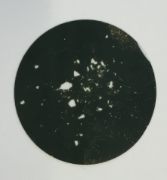
\includegraphics[width=.7\linewidth]{glass}
  \label{cross}
\end{subfigure}%
\begin{subfigure}{.5\textwidth}
  \centering
  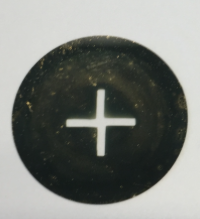
\includegraphics[width=.7\linewidth]{cross}
  \label{glass}
\end{subfigure}
\caption{A few examples of the \diameter 25 mm glass slides with a golden layer on top of it. Left: the transparent areas created with the help of small pieces of glass. Right: with the use of small iron crosses a transparent area with the form of a cross was created.}
\label{gold_layer}
\end{figure}

\begin{figure}[ht!]
\centering
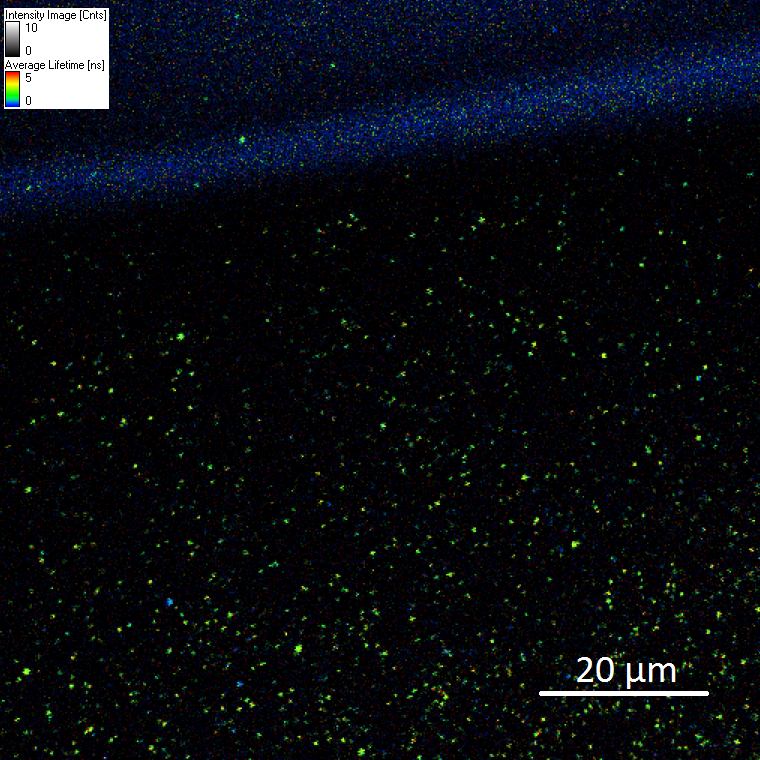
\includegraphics[width=\textwidth]{border_legenda}
\caption{(80 x 80) $\upmu \textup{m}^{2}$ image of the slim border. The top part of the image is gold, the bright blue line is the border between the gold and the glass and the green spots below the border is azurin.}
\label{border}
\end{figure}

The latter method to create reliable areas is used in the next phase of the experiment: the combination of the electron mediator, proteins and the gold layer. Individually these parts worked as intended. However, a combination of the parts lead to two serious problems:
\begin{enumerate}


\item Damaged gold layer.
The longer the experiment continued, the more clear it was that the border of the goldlayer would slowly seperate. At the end of a day of experiments, the gold layer was damaged to such an extend that it would simply seperate from the sample slide. The PES is most likely the reason for this. Though the exact reason for this was never clear - when a golden layer was exposed to a different electron mediator (ferricyanide or ascorbate) the gold layer seemed to be not damaged. The damage caused by PES can be seen if you compare the border of the gold layer (bright blue) of Figure \ref{no_prot} - taken at the start of the experiment -  with the border of Figure \ref{damaged_border} (this picture was taken towards the end of a day of experiments). One way to tackle this problem, as suggested by one of the professors, would be a protective layer on top of the gold layer. This protective layer is 4-Mercaptobutanoic acid ($\textup{C}_{4}\textup{H}_{8}\textup{O}_{2}\textup{S}$). This kind of protective layer has been used in similar experiments \cite{Elmalk2012} where it has been shown that the length of the carbon chain can vary without effecting the electron exchange between the gold and the single molecule. In these experiments, however, usually the molecules were on top of the gold layer whereas in our case the proteins are next to the gold layer. The result of using this protective layer was that the proteins did not show any redox, even when different potentials were applied. Since the protective layer did not work, the other way to tackle the damaged gold layer is an increase in thickness of the gold layer. This will not solve the problem, but delay it long enough to do proper experiments. In all previous experiments, the thickness of the gold layer was 20nm. Increasing the thickness of the gold layer led to the second problem.

 \begin{figure}[ht!]
\centering
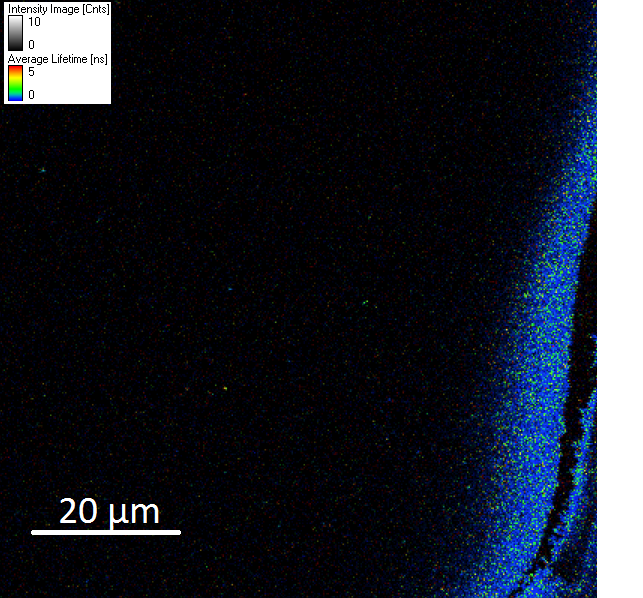
\includegraphics[width=\textwidth]{damagedborder}
\caption{(80 x 80) $\upmu \textup{m}^{2}$ of the bright blue border between gold (far right) and glass (left), showing the fractured border due to PES damaging the golden layer.}
\label{damaged_border}
\end{figure}

\item Missing proteins.
Near the edges of the working electrode, a much lower density of proteins was observed (see Figure \ref{no_prot}) once the gold layer thickness was increased. The reason for this could be that during the sputtering of the gold layer, the metal crosses would slightly move a little bit and thus damaging the methoxy-peg-NHS layer. This would make it harder for proteins to bind near the surface. Another explanation could be the fact that some gold-particles might have slipped under the metal cross and taking the spots where the proteins usually would bind. 


\begin{figure}[ht!]
\centering
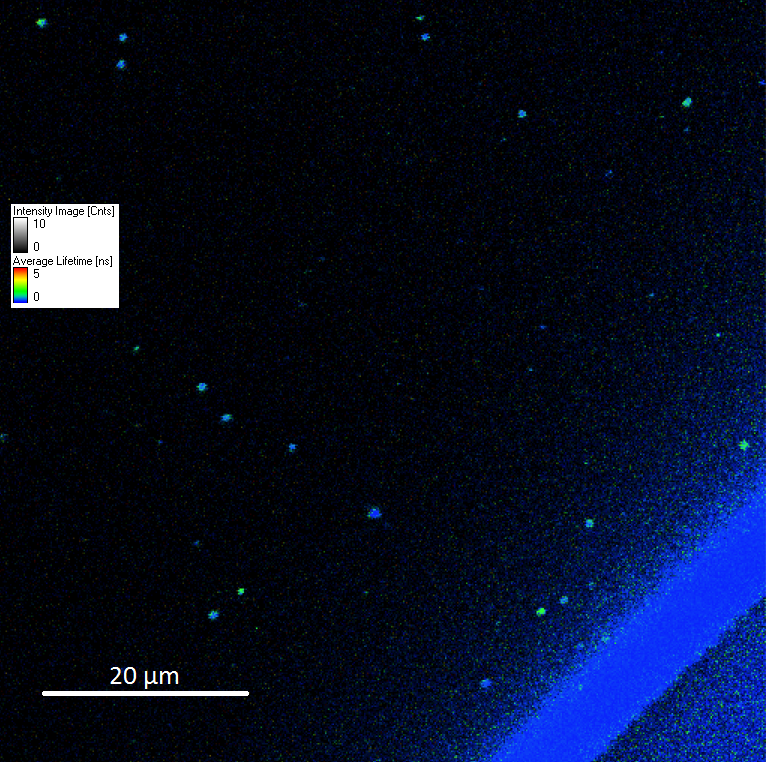
\includegraphics[width=\textwidth]{no_prot}
\caption{The (80 x 80) $\upmu \textup{m}^{2}$ of the glass surface near the 200nm thick golden layer. As can be seen, almost no proteins are present despite using the same molecule densities.}
\label{no_prot}
\end{figure}

\end{enumerate}

\subsection*{The final setup: platinum grid} \label{grid_1}
At this point of the process it was clear that the gold-layer as a working electrode in the current setup gave too many problems and a final solution was attempted. Instead of using a gold layer, a single golden wire was kept on the sample slide to see if this would give any good results. This can be seen in Figure \ref{goldenwire_1}. The green color are the proteins showing switching and blinking. This was the first sign that instead of the golden layer, a (golden) wire as working electrode could do the trick.  Finding a single wire with the microscope and keeping it on the sample slide is a tough task and is not controllable and thus a change was needed. Instead of one golden wire, a platinum rectangular grid (the total length/width of the grid is around 2.5 cm) is used and pressed on the sample slide with the help of a small glass slide. Not only is the pressure evenly applied on the grid when pressure is applied on the glass slide on top of the grid, but also small confined volumes are formed where the sample slide and glass slide form the 'floor' and 'roof' and the platinum grid the 'walls'. These confided volumes are in the order of nanoliters, which makes switching possible in a matter of minutes. On top of changing the working electrode, also the electron mediator was changed. Once the setup worked, PES showed more disadvantages such as its very high autofluorescence which makes the ratio signal-to-noise very low. PES is hydrophobic and is difficult to mix with the PBS: it will get stuck on the surface and interacts with the proteins. To avoid these problems a different electron mediator is used in the final experiments. A mixture of 200 $\upmu \textup{M}$ ferricyanide and 100 $\upmu \textup{M}$ ascorbate mixed with PBS to a total volume of 4 mL. This was the last step in order to make the whole setup work as intended. The setup is schematically drawn in Figure \ref{final_setup} with a short description of its parts.


\begin{figure}[ht!]
\centering
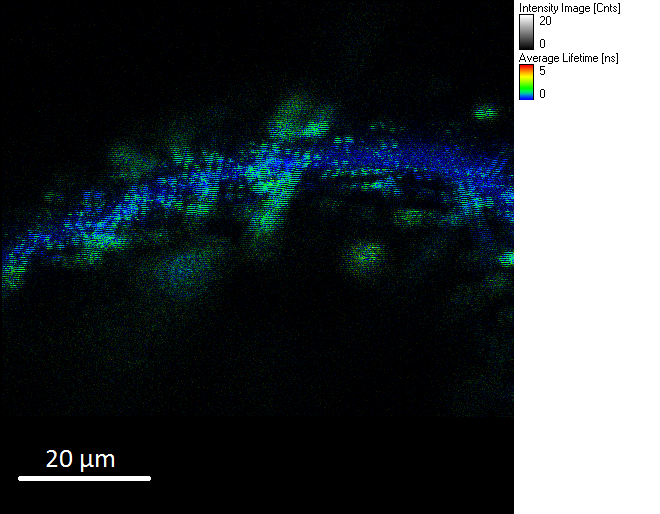
\includegraphics[width=\textwidth]{goldwire_1}
\caption{A (80 x 80) $\upmu \textup{m}^{2}$ area of the sample slide with immobilized proteins. The blue 'snake' is the golden wire that touches the sample slide. The green spots represent the oxidized proteins. This is the first proof that proteins near the wire show oxidation.}
\label{goldenwire_1}
\end{figure}


\begin{figure}[ht!]
\centering
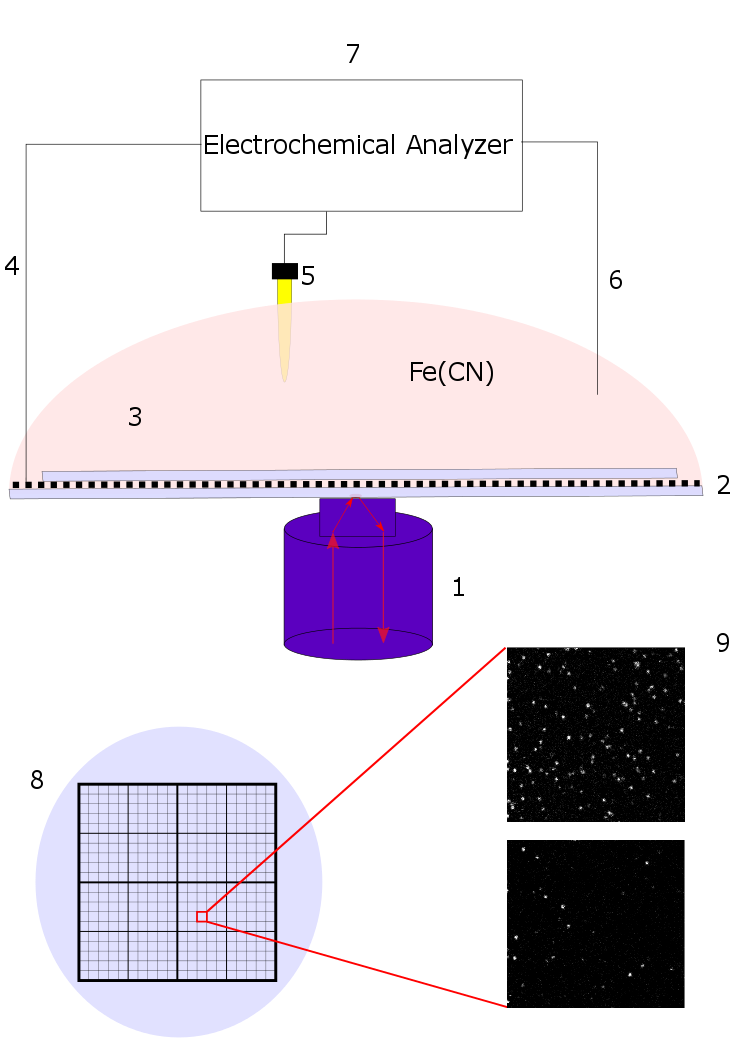
\includegraphics[width=.75 \textwidth]{final_setup}
\caption{Not to scale schematic picture of the final setup in which the potential is changed electrically. \textbf{(1)} The confocal microscope as described at the beginning of this chapter. \textbf{(2)} The functionalized sample slide with on top the platinum grid and another small glass slide to press the grid on the sample slide, resulting in small confined volumes in the order of nanoliters. \textbf{(3)} The electron mediator consistent of 200 $\upmu \textup{M}$ ferricyanide, 100 $\upmu \textup{M}$ ascorbate and PBS (PH 7.4) with a total volume of 4 mL. \textbf{(4)} The working electrode (golden wire) in connection with the platinum grid (section \ref{grid_1}). \textbf{(5)} The saturated calomel reference electrode. \textbf{(6)} A platinum wire, not touching the grid, as the counter electrode. \textbf{(7)} The electrochemical analyzer ( Model 800B Series Electrochemical Detector, CH Instruments) to which the electrodes are connected. \textbf{(8)}, \textbf{(9)} Top view of the sample slide and two pictures of the same area showing the same CuAz reduced and oxidized.}
\label{final_setup}
\end{figure}

\chapter{Results and discussion}

The experiments were performed with the blue copper protein azurin from Pseudomonas aeruginosa, labeled with ATTO655 (refered to as CuAz in the rest of the analysis). This small protein, with a molecular mass of 14 kDa, is involved in electron transfer (ET) reactions in a variety of both plants and bacteria. Its label, ATTO655, has been chosen since its properties have been well documented \cite{pvd_11}. The labeling site used in this experiment is K122 (lysine at position 122), one of the closest labeling sites to the copper center of CuAz. In the future one could label ATTO655 to a labeling site further from the copper so that the inner-dye distance changes from less to greater than the F\"{o}rster radius $R_{0}$ value for maximal sensitivity \cite{Roy2008}. 
Beside the blue copper protein azurin, fluoresecntly labeled zinc azurin (ZnAz) was also used to perform experiments. This wild-type protein is used as a control since it does not show fluorescence switching when different potentials are applied.

\section*{Data collection} \label{data_coll}
The sample, mounted on the scanning stages, was brought into the focal plane of the objective. Once an areas was chosen, images of (80 x 80) ($\upmu \textup{m}^{2}$) were recorded as x-y scans. A positive and negative potential is applied and captured to detect the blinking CuAz. Images of typically (20 x 20) ($\upmu \textup{m}^{2}$) were recorded in which at least 10 blinking molecules were present. To collect data from a single molecule, the laser was parked on the blinking molecule and measurements were made for 30 seconds. Once all the blinking molecules of interest were measured, a new potential was applied and this process repeated. Many fluorophores bleach within seconds, thus only the timetraces of those molecules who survived all the different potentials were included for further analysis. 

To make sure that the surroundings of the singe molecules were indeed the intended potential, the I-t curves were recorded at the same time. Once the I-t curves stay constant, it is assumed that the solution has the same potential as the potentiostat applies. Two examples of these I-t curves are shown in Figure \ref{it_curves}

\begin{figure}[ht!]
\begin{subfigure}{.5\textwidth}
  \centering
  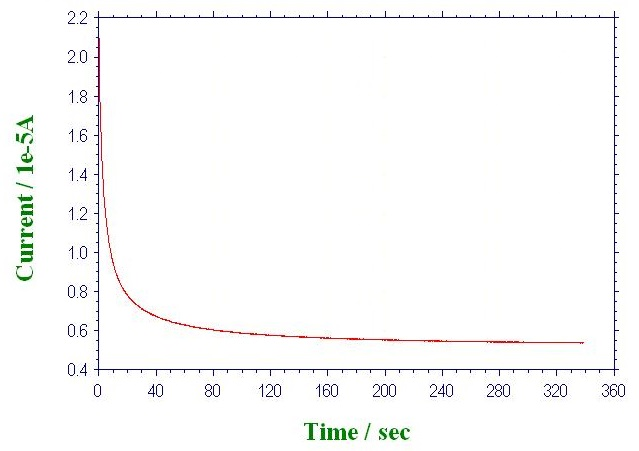
\includegraphics[width= \textwidth]{it25mV}

  \label{}
\end{subfigure}%
\begin{subfigure}{.5\textwidth}
  \centering
  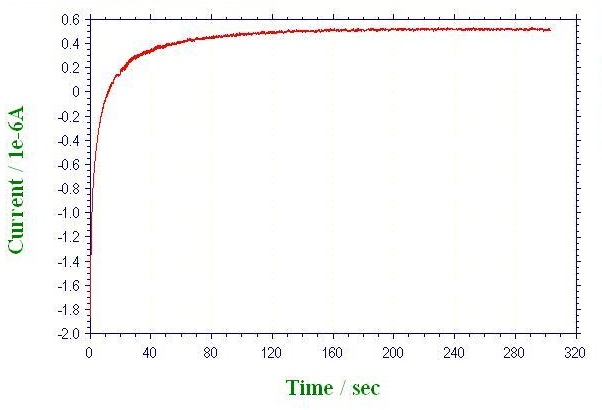
\includegraphics[width=.95 \linewidth]{it100mV}
  \label{}
\end{subfigure}
\caption{The amperometric i-t curve.  Right: the i-t curve of reducing conditions (-25 mV applied in this case). Left: the I-t curve of oxidizing conditions (100 mV applied in this case).}
\label{it_curves}
\end{figure}


\section*{Timetrace analysis}
The software used for the fluorescence lifetime imaging and correlation software is SymPhoTime 64. With the help of this program, timetraces and its specific parameters are saved in .pt3 files. Older versions of SymPhoTime saved this data into .t3r files. Previous PhD student .. had written a program in MATLAB R2012b and C++ to read out the .t3r files and transfer the timetraces into multiple .dat files. This program has been adjusted in such a way it can read out the .pt3 files from the newer version of SymPhoTime 64. It allows you to manually select parts of the timetrace, as is shown in Figure \ref{timetrace_selection}.

\begin{figure}[ht!]
\centering
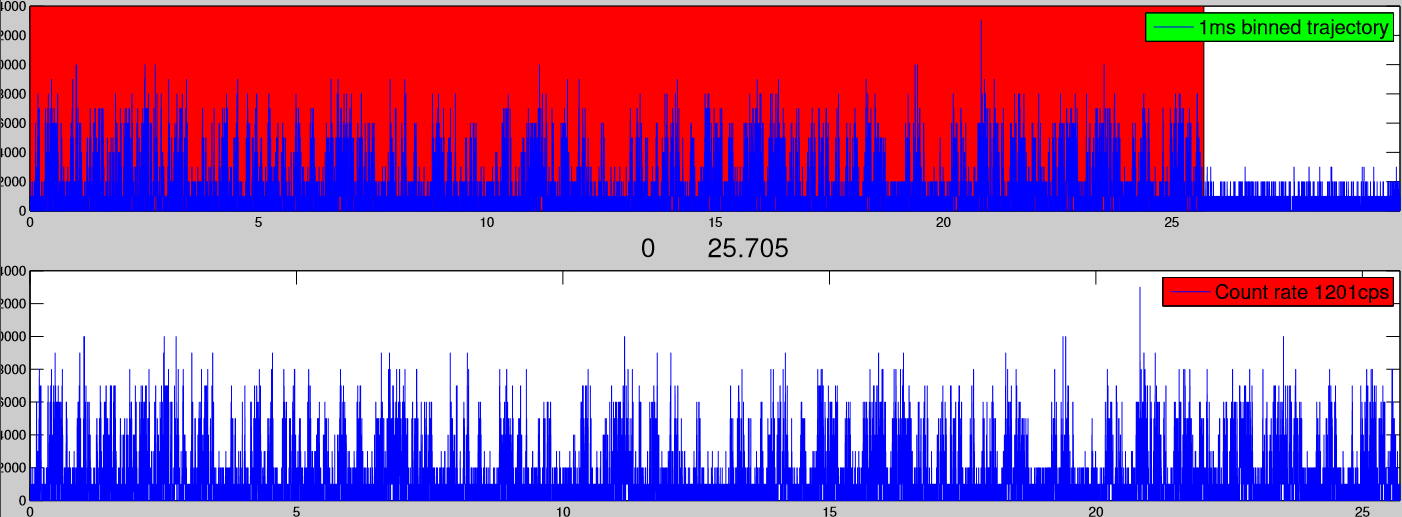
\includegraphics[width=\textwidth]{timetrace_selection}
\caption{Selection of a timetrace with a program written in MATLAB R2012b and C to select the parts of the timetrace (in red) that will be put into .dat files. As in this specific case the Cu-Azurin bleached around 25.7 second mark and the timetrace once it is bleached is not of interest and therefore not selected.}
\label{timetrace_selection}
\end{figure}

Once the timetrace is selected and put into several .dat files, another C program is run to precisely calculate the  on- ($\tau_{on}$) and off times ($\tau_{off}$). This program uses several mathematical methods to calculate the timestamps and intensity of intensity jumps in optical single molecule emission data that exhibit discrete intensity jumps, in detail described by Lucas P. Watkins and Haw Yang in their paper \cite{And2004}. As an example, several on- and off times are visualized in Figure \ref{on_off_times}. These times are defined as the duration of the CuAz being oxidized ($\tau_{on}$) and reduced ($\tau_{off}$). The intensity jumps that are controlled is what is referred to as 'switching' while the (often) unwanted and uncontrolled switching between the bright 'on' and dark 'off' states is called 'blinking'. 

\subsection*{Results and discussion timetraces CuAz}

Looking at the timetraces between 100mV and 0mV (Figure \ref{plots_timetraces_diff_pot}) a trend is noticeable on sight. For the higher potentials, the $\tau_{off}$ are long and the $\tau_{on}$ are relatively short which goes hand in hand with the low amount of events. When the potential decreases the amount of events start to increase and the $\tau_{on}$ becomes longer while $\tau_{off}$ becomes shorter. The explanation for this is simply the FluRedox principle. CuAz in oxidized form (copper is in $\textup{Cu}^{2+}$) shows an absorbence maximum around 628nm which overlaps with the fluorescence emission of the ATTO655 dye as is shown earlier in Figure \ref{absorption}. Since FRET is high in this form, the fluorescence of the dye is quenched resulting in longer $\tau_{off}$. When the potential is decreasing, the solution is reducing. When CuAz is reduced - since the absorption at 628nm disappears upon reduction - the FRET is low and thus the dye  shows high fluorescence and longer $\tau_{on}$ times are expected. This principle seems to be the only role in play until the potential comes near 25mV. Here a new phenomenon is noticeable. Beside the expected  increasing $\tau_{on}$ and decreasing $\tau_{off}$ due to switching of CuAz, a secondary timescale seems to be shown in the form of very short $\tau_{on}$ in very short succession. To explain this event, a closer look has to be taken at the chemicals involved in the chemical processes concerning the redox reactions. Apart from the intramolecular electron transfer between the label and the copper center, intermolecular reactions between the redox active components in the solution and the dye are also present. For higher potentials, the time scale of the events between dye and solution are relatively high. When the potential gets lower, the solution is more and more reduced. The interaction between the dye and the reduced ascorbate and ferricyanide happen on a smaller timescale and is now prominent in the timetraces. This is more apparent when looked at the autocorrelation. The probability $I(t)$ of emission of a photon by an excited state at time t is determined by
\begin{equation} \label{solt}
dI(t) = -\frac{1}{\tau(t)}I(t)dt.
\end{equation}
The solution of equation \ref{solt} in the case of $\tau(t) = \tau_{0}= constant$ is the classical single exponential decay function. At higher potentials the autocorrelation can be fitted with this single exponential in the form of
\begin{equation} \label{single_exp}
g(\tau) =  A_{1}e^{-\tau/t_{1}}
\end{equation}
where $t_{1}$ and $A_{1}$ are constants. These constants are related to the on- and offtimes via the equations
\begin{equation}\label{tau_on}
\tau_{on} = t_{1} +\frac{t_{1}}{A_{1}}
\end{equation}
and
\begin{equation}\label{tau_off}
\tau_{off} = t_{1} +t_{1}A_{1}.
\end{equation}
When the potential is lowered towards the 25 mV and below, a single potential does not fit the autocorrelation but rather a sum of two exponentials fits the autocorrelation: 
\begin{equation}\label{multi_exp}
g(\tau) = A_{1}e^{-\tau/t_{1}} + A_{2}e^{-\tau/t_{2}}. 
\end{equation}
The constant-pair $t_{1}$ and $A_{1}$ and $t_{2}$ and $A_{2}$ are related with the on- and off-times according equation \ref{tau_on} and equation \ref{tau_off}. The longer $\tau_{on}$ are the ones from the switching of the CuAz, while the shorter $\tau_{on}$ is the one due to the blinking of the dye.


\begin{figure}[ht!]
\centering
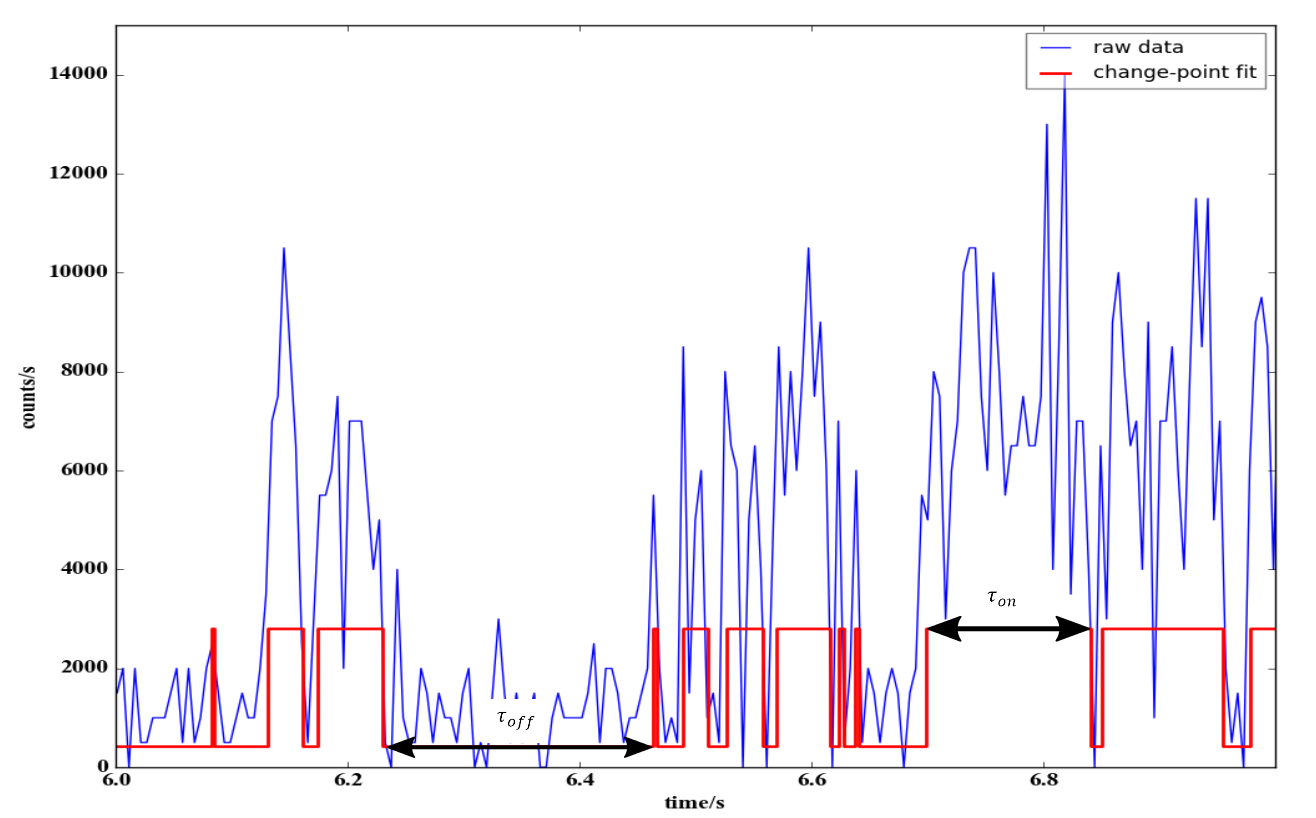
\includegraphics[width=\textwidth]{on_off_test1}
\caption{Same timetrace as Figure \ref{timetrace_selection} but a smaller range. In red is plotted the calculated intensity jumps according to the program written by Lucas P. Watkins and Haw Yang. The time when the intensity is low is referred to as the $\tau_{off}$ and the time the molecules intensity is high is the $\tau_{on}$.}
\label{on_off_times}
\end{figure}

\begin{figure}[ht!]
\centering
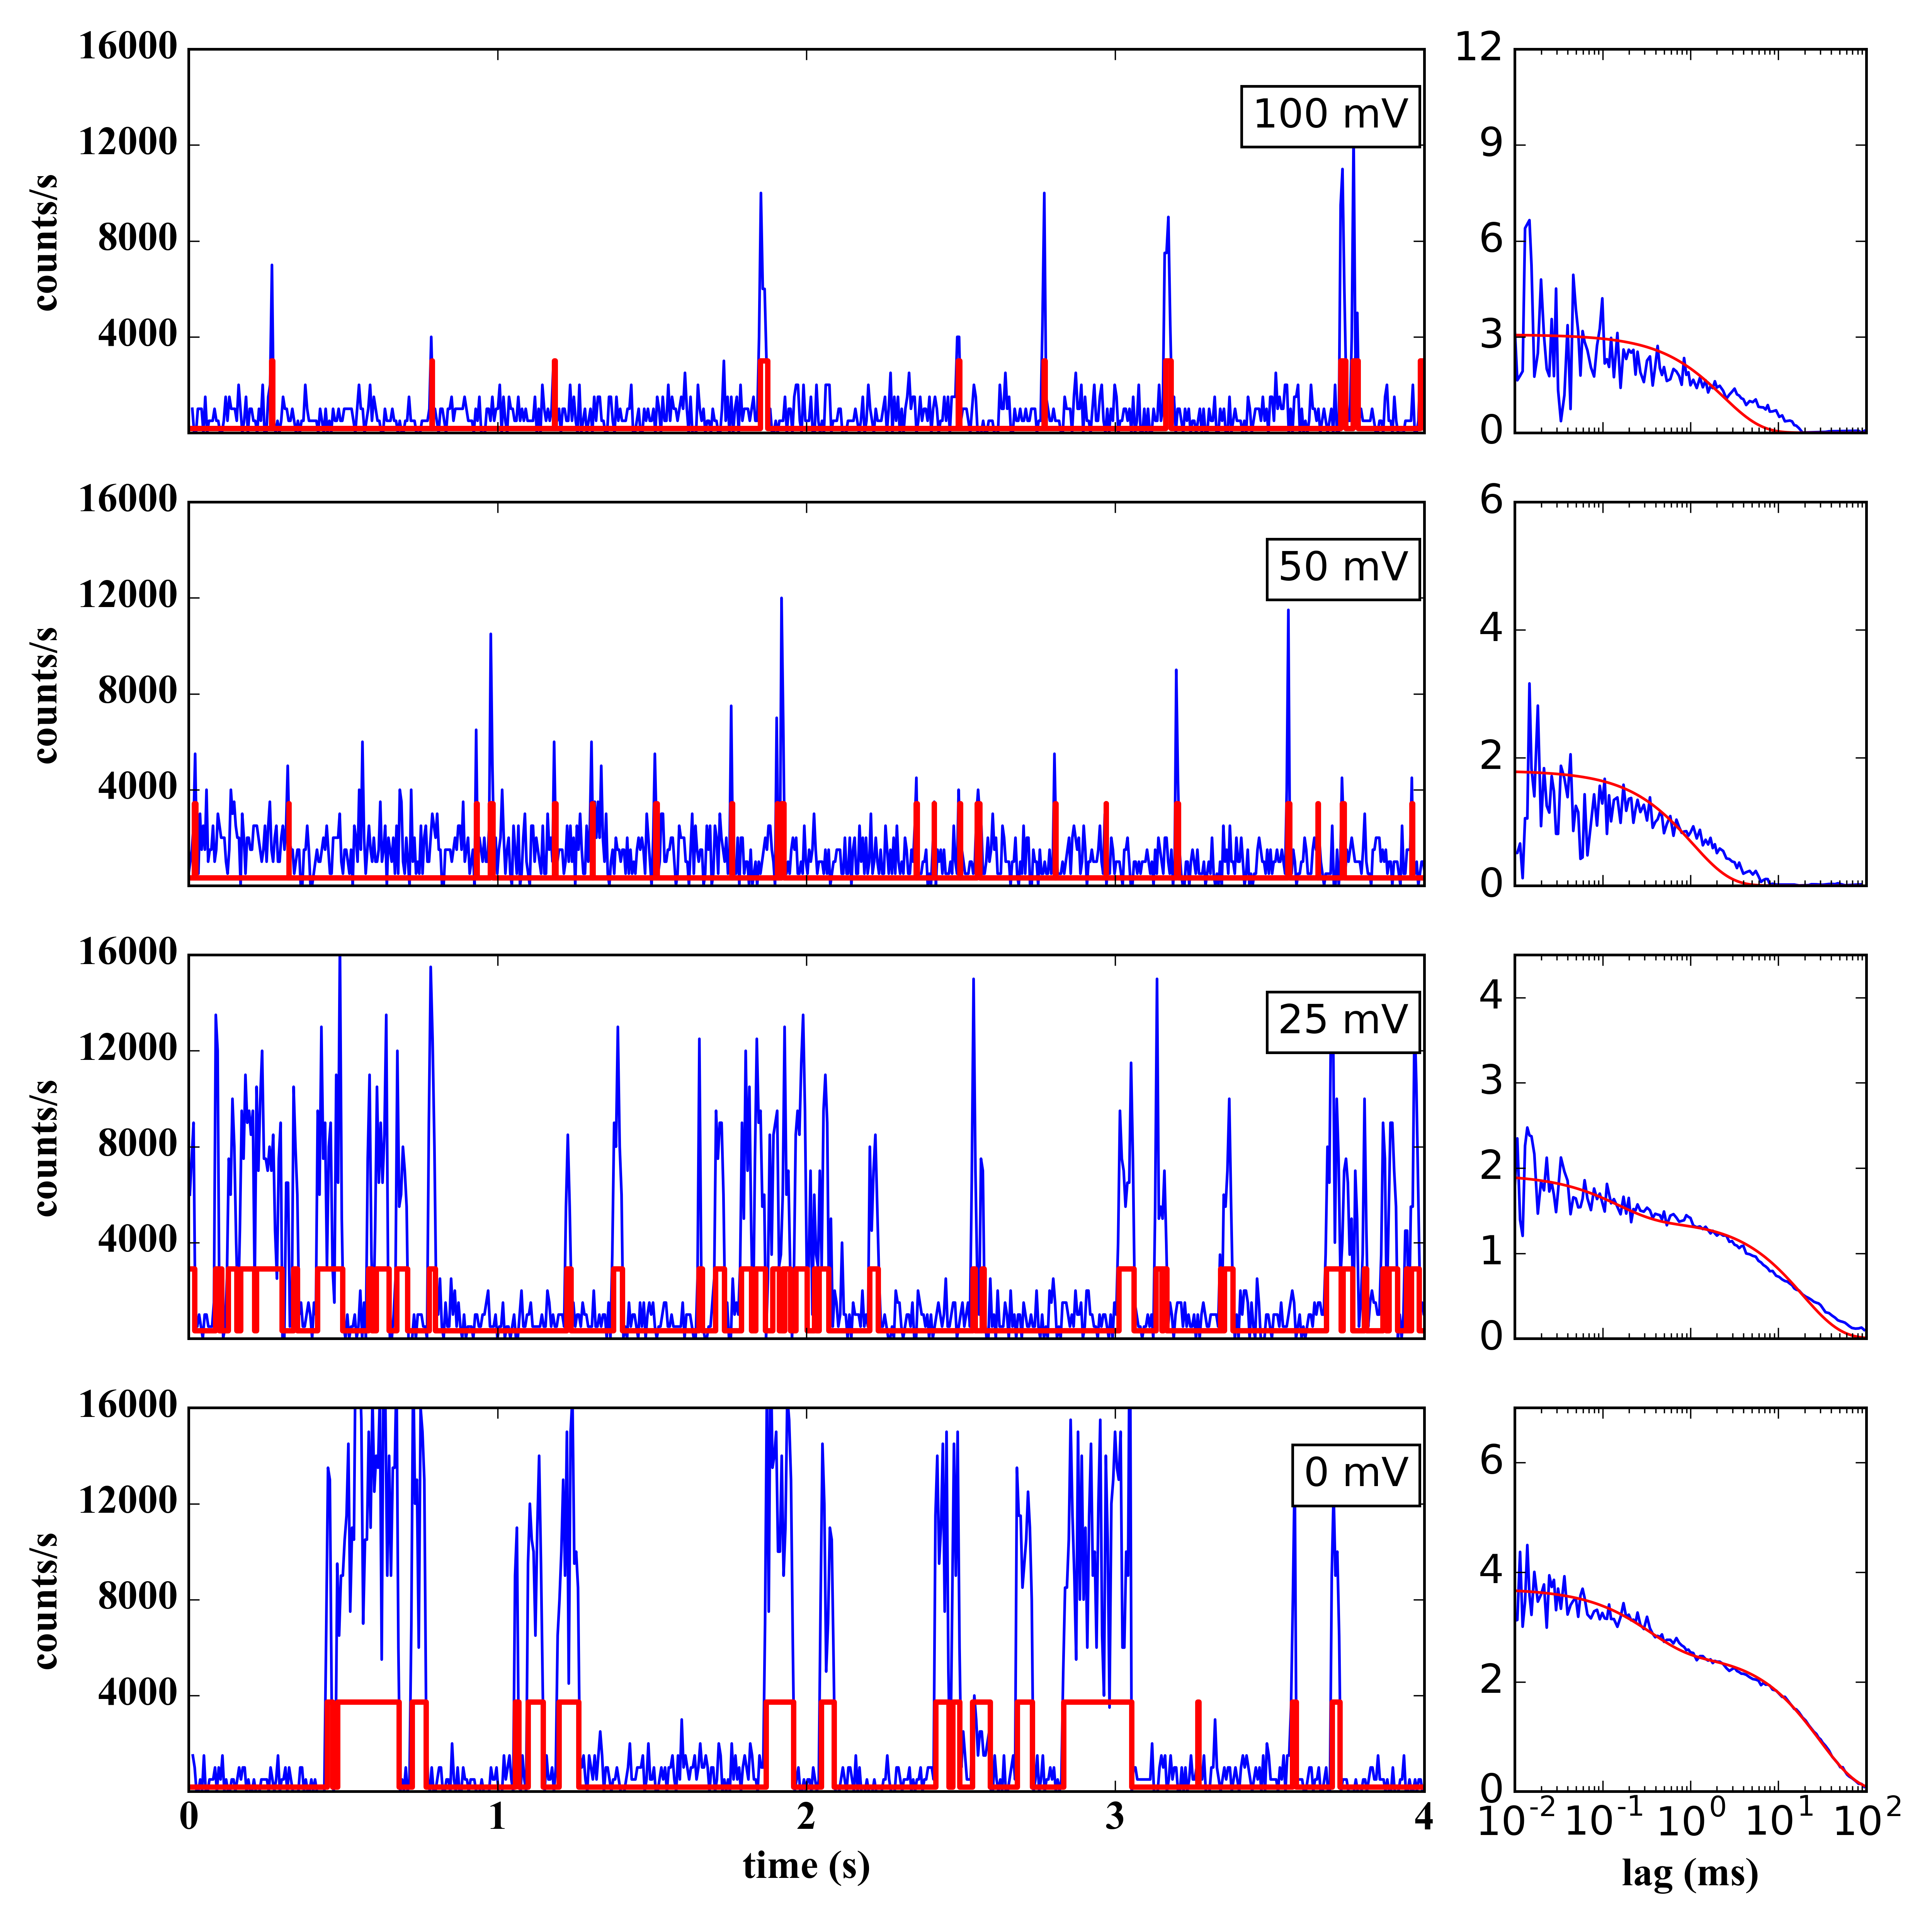
\includegraphics[width=1\textwidth]{plots_timetraces_diff_pot}
\caption{Timetraces together with its autocorrelation of the same CuAz molecule under different potentials. A clear difference between $\tau_{on}$ and $\tau_{on}$ under different potentials is visible: shorter $\tau_{on}$ for higher oxidizing potentials, longer $\tau_{on}$ for reducing lower potentials. For potentials below 25mV this pattern gets disturbed due to blinking of the ATTO665. This phenomenon is shown in the autocorrelation by changing from a single exponential fit to a multi-exponential fit.}
\label{plots_timetraces_diff_pot}
\end{figure}



Another way of looking at the $\tau_{on}$ and  $\tau_{off}$ is by plotting the distribution of the on and off times in the timetraces. This is done in Figure \ref{histograms_disc}. The fit through these histograms will give the average on- and off-times. A very interesting phenomenon is observed in the off-times however. Where the on-times are fitted with a single exponent, the off-times have a different form. Very short off-times seem to be relatively rare. To get a deeper understanding of this a closer look has to be taken at the electron transfer process between the solution and the copper azurin.
\begin{equation}\label{ox_pros}
\textup{Cu}^{2+}\xleftarrow[3]{\overset{1}{\longrightarrow}\textup{Cu}^{2+}+ e^{-}\overset{2}{\longrightarrow}}\textup{Cu}^{1+}
\end{equation}
The reduction of $\textup{Cu}^{2+}$ to $\textup{Cu}^{1+}$ is a multi-step process. Bringing the electron close to the copper center (step 1) and reducing the copper (step 2) is happening in two short time scales. Contrary to the reduction of copper azurin, the oxidation is a single step process. This should go faster than reducing and thus shorter off times are expected to be much more present. This is in contradiction to the histograms which show an absence of these short times. Something in step 3 is delaying the oxidation. With the model presented above, this cannot be explained and further research to this subject is needed.

\begin{figure}[ht!]
\centering
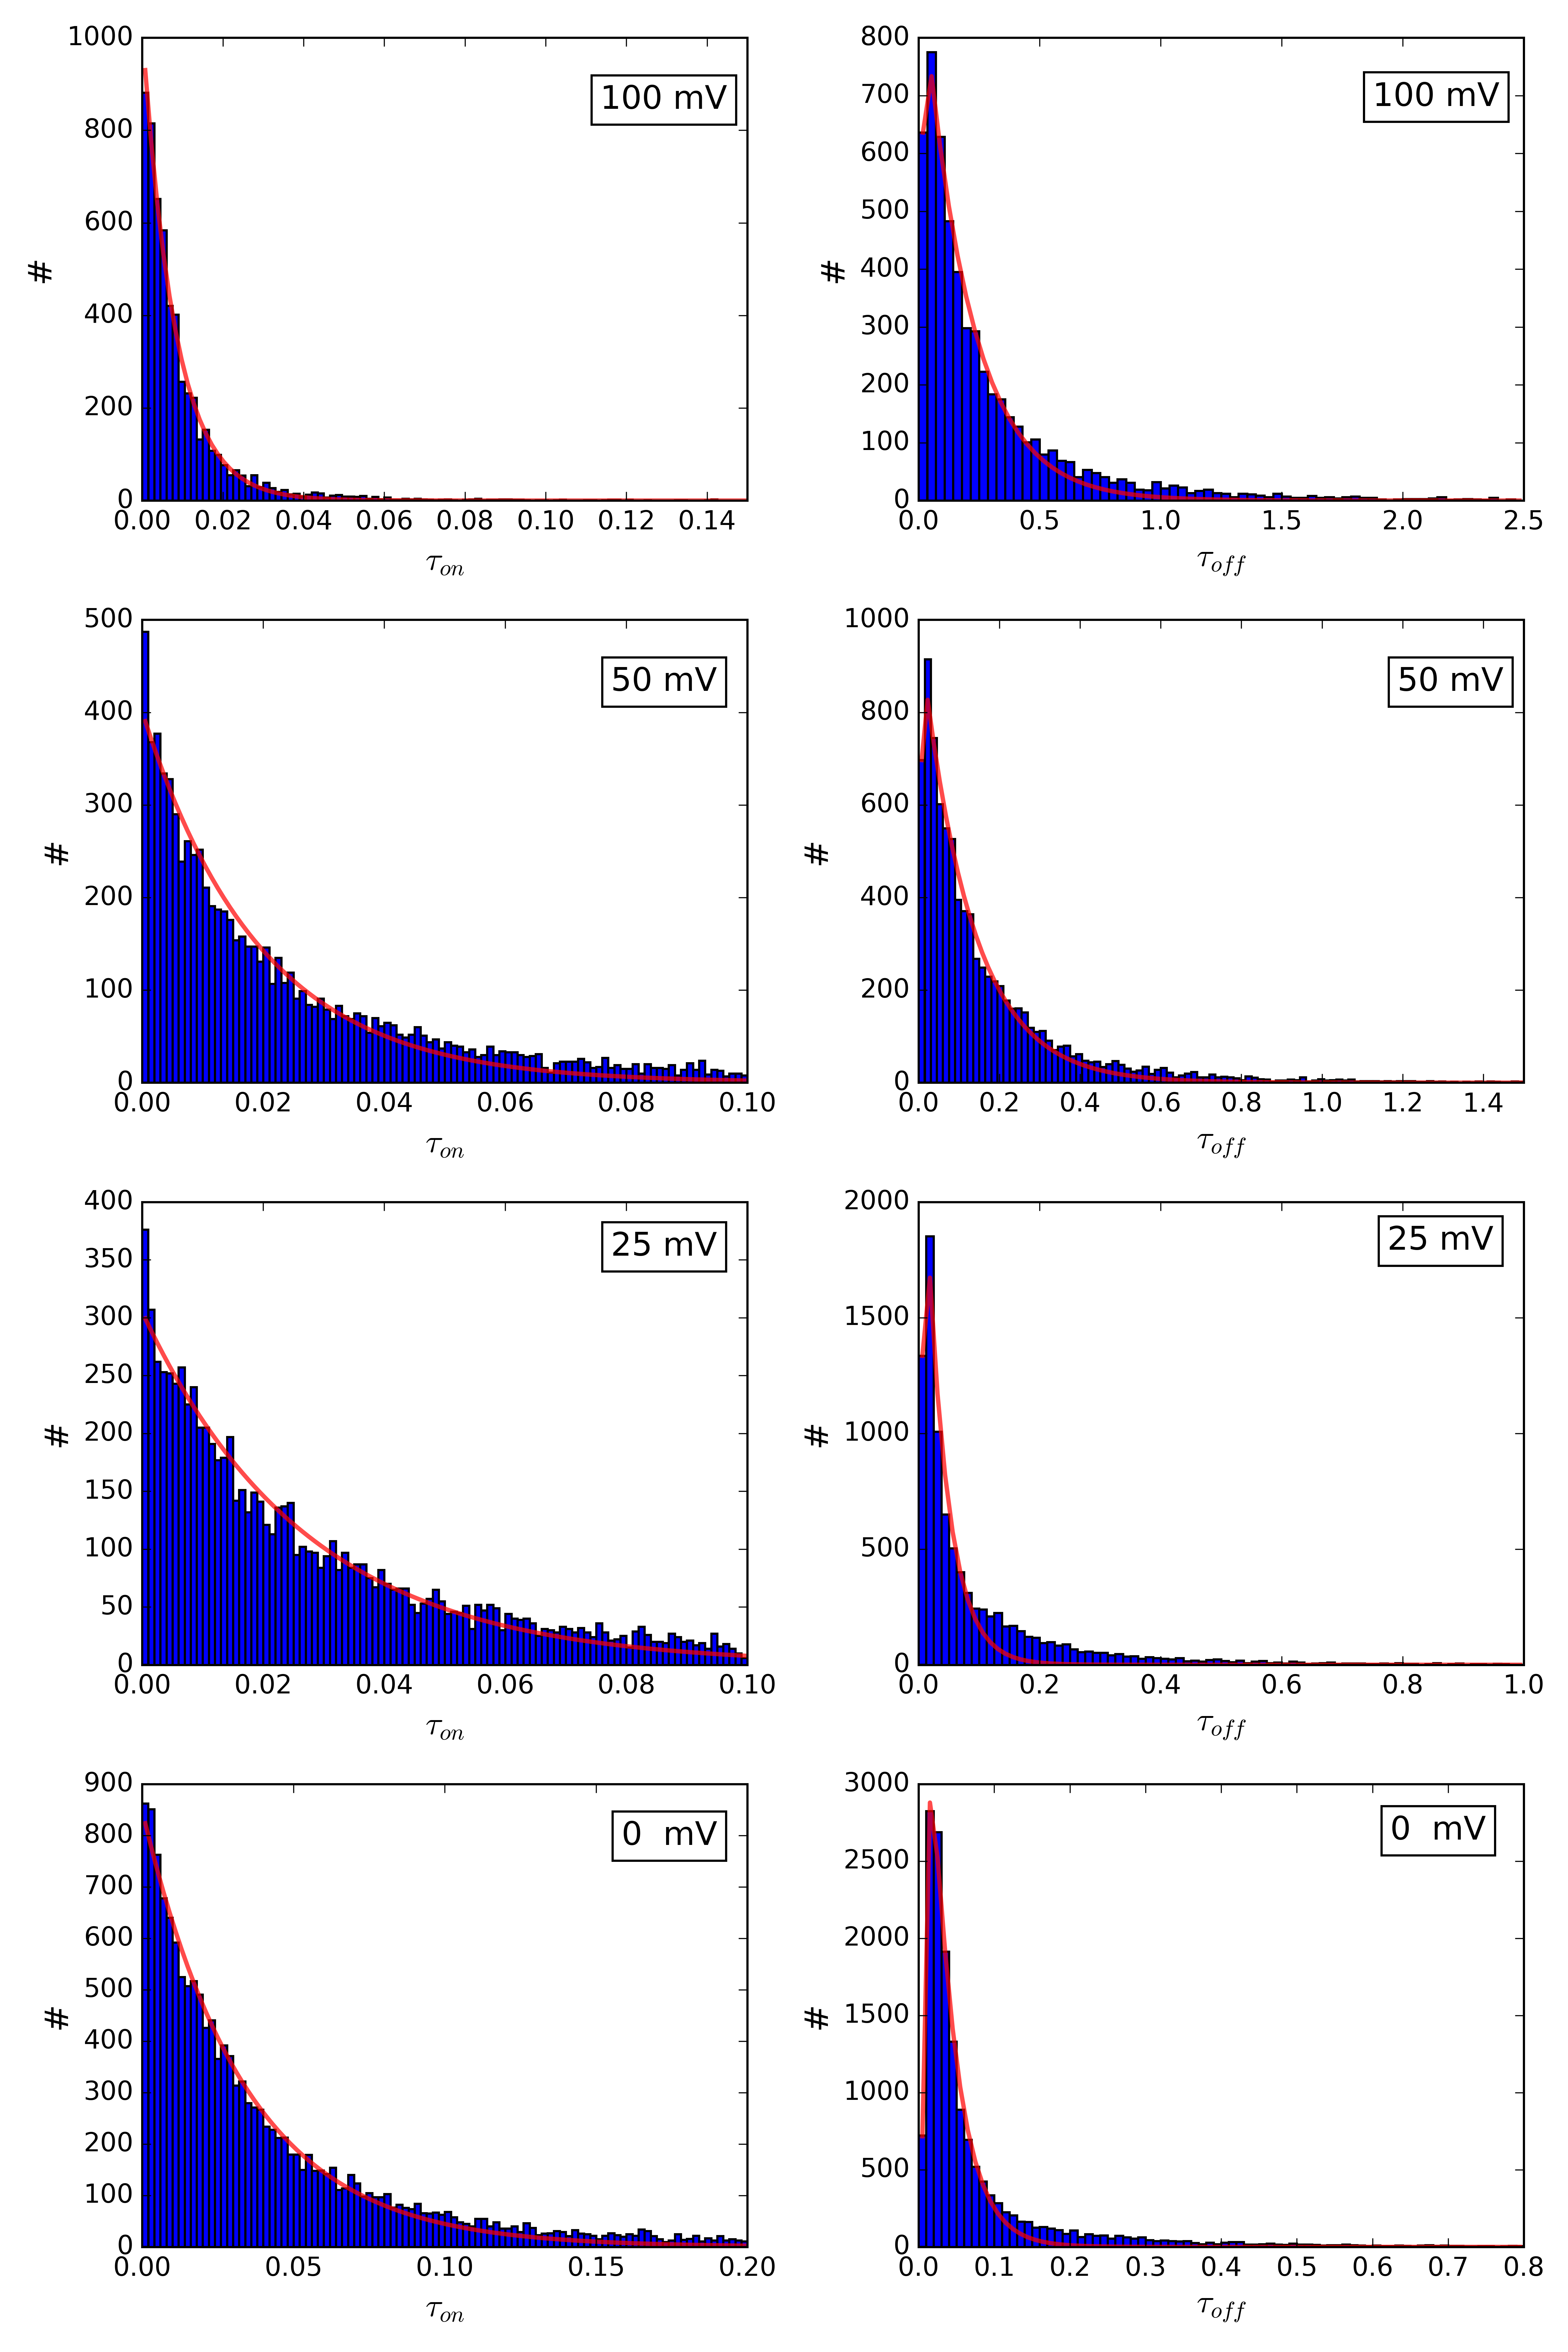
\includegraphics[width=.9\textwidth]{histograms_thesis}
\caption{Histogram distribution $\tau_{on}$ and $\tau_{off}$ at different potentials.}
\label{histograms_disc}
\end{figure}

To give the switching of the CuAz a more quantitatively meaning, the average $\tau_{on}$ ($\bar{\tau}_{on}$) and average $\tau_{on}$ ($\bar{\tau}_{off}$) can be related to the Nernst equation since the switching is due to the redox reaction of CuAz. Rewriting equation \ref{nernst} to 

\begin{equation}\label{nernst_tau}
E = E_{0}+\frac{k_{B}T}{ne}\textup{ln}\frac{\bar{\tau}_{off}}{\bar{\tau}_{on}}
\end{equation}
the average on- and off-times can be related to the potential applied. Rewriting equation \ref{nernst_tau} leads to
\begin{equation}\label{fit_onoff}
\frac{\bar{\tau}_{off}}{\bar{\tau}_{on}} = \textup{exp}\left ( \frac{E_{0}-E}{0.059} \right ).
\end{equation}
A fit through the ratio of the $\frac{\bar{\tau}_{off}}{\bar{\tau}_{on}}$ and the applied potential $E$ will lead to the midpoint potential $E_{0}$ of the protein. The on- and off-times above 30 mV are extracted directly from the timetraces. For the potentials below 30 mV, the on- and off-times are extracted from the autocorrelation. Since the fit for the autocorrelation consist of two exponentials, the exponent in which the $\tau_{on}$ has the smallest value is considered to be the one belonging to the blinking of the dye. Using this rule the ratio $\frac{\bar{\tau}_{off}}{\bar{\tau}_{on}}$ that belongs to the CuAz can be determined for values below the 30 mV. Using the data of one experimental day: 19 different protein under at least 8 different potentials between 0 mV and 100 mV, the midpoint potential is determined to be 25.62 mV. This is in accordance with the 25 mV given in other literature (citation needed). 

\begin{figure}[ht!]
\centering
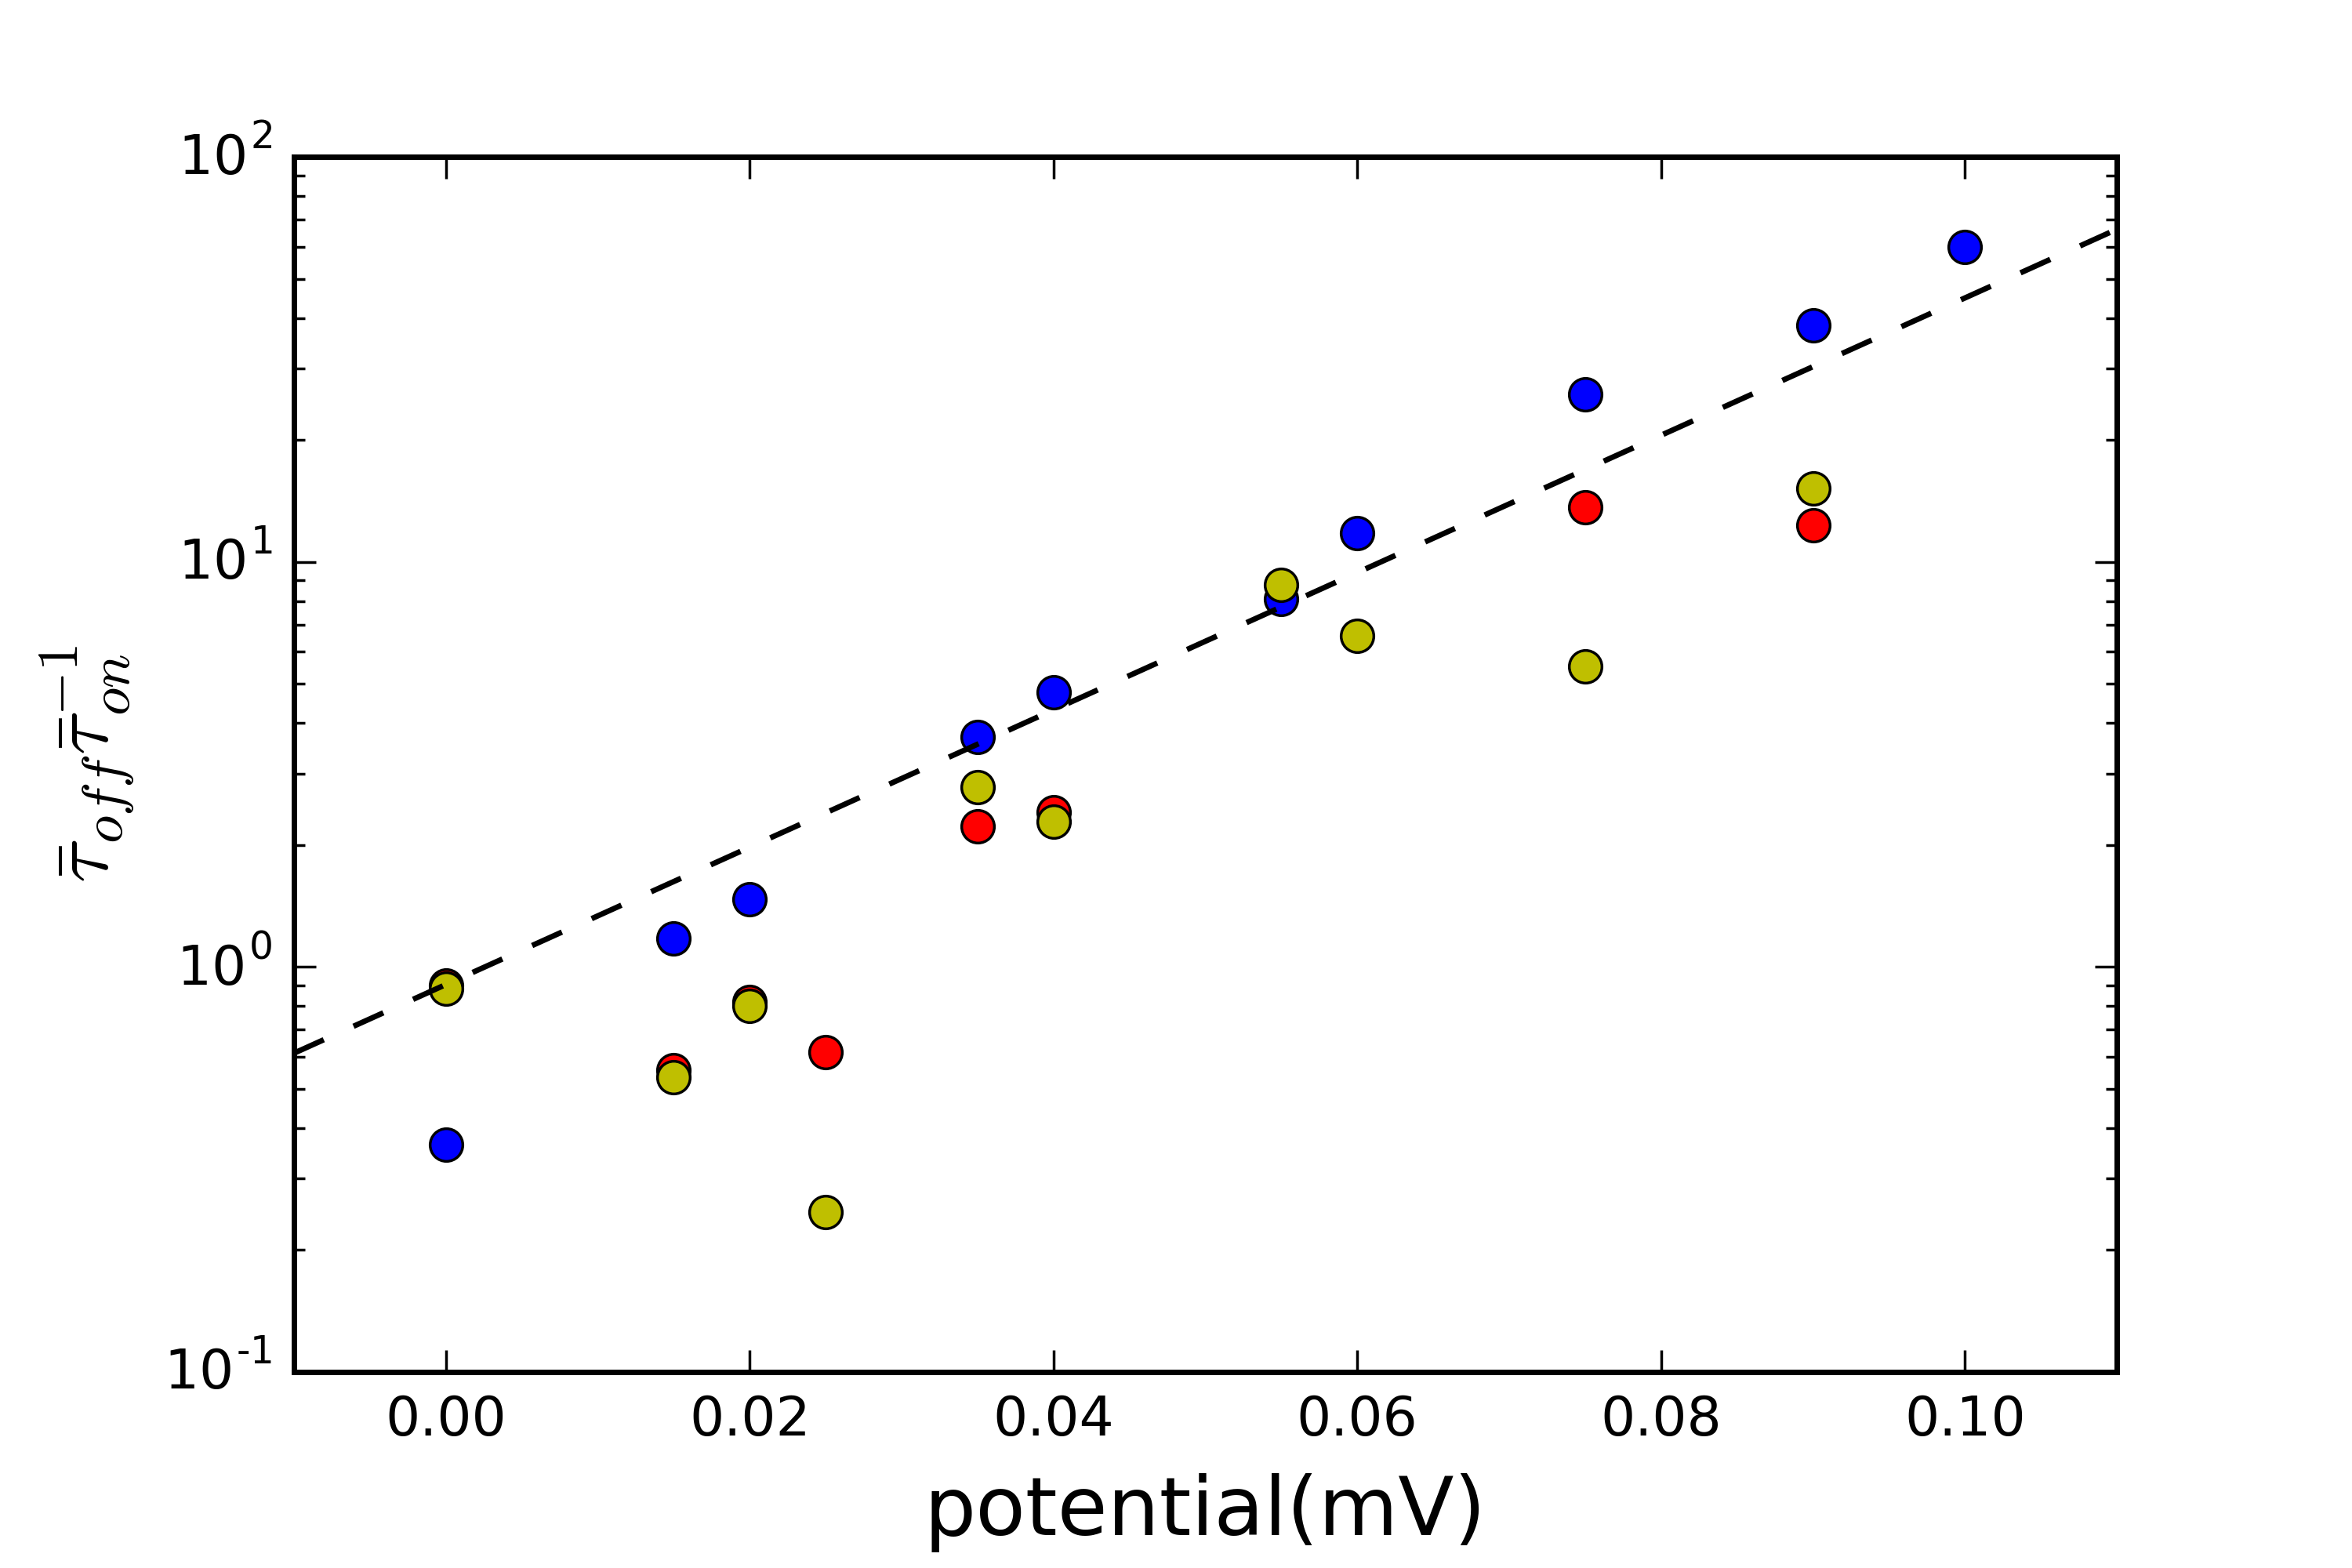
\includegraphics[width=.9\textwidth]{t_ratio_plot}
\caption{Plot of the ratio of $\frac{\bar{\tau}_{off}}{\bar{\tau}_{on}}$ versus the potential of three different CuAz proteins (each represented with a different color). The dashed black line is the average fit of 15 different single CuAz molecules.}
\label{t_ratio_plot}
\end{figure}

\bibliographystyle{lion-msc}
\bibliography{THESIS}

\end{document}
